\chapter{Appendix}

\section{Line Candidate Cutouts}\label{sec:A1}

The following plots show the 35 CO line candidates in various wavelengths. The red contours show the +2$\sigma$,4$\sigma$,6$\sigma$,and 8$\sigma$ values in the datacubes. All cutouts are 3x3 arcseconds in size.

\begin{figure}[tbp]
\centering 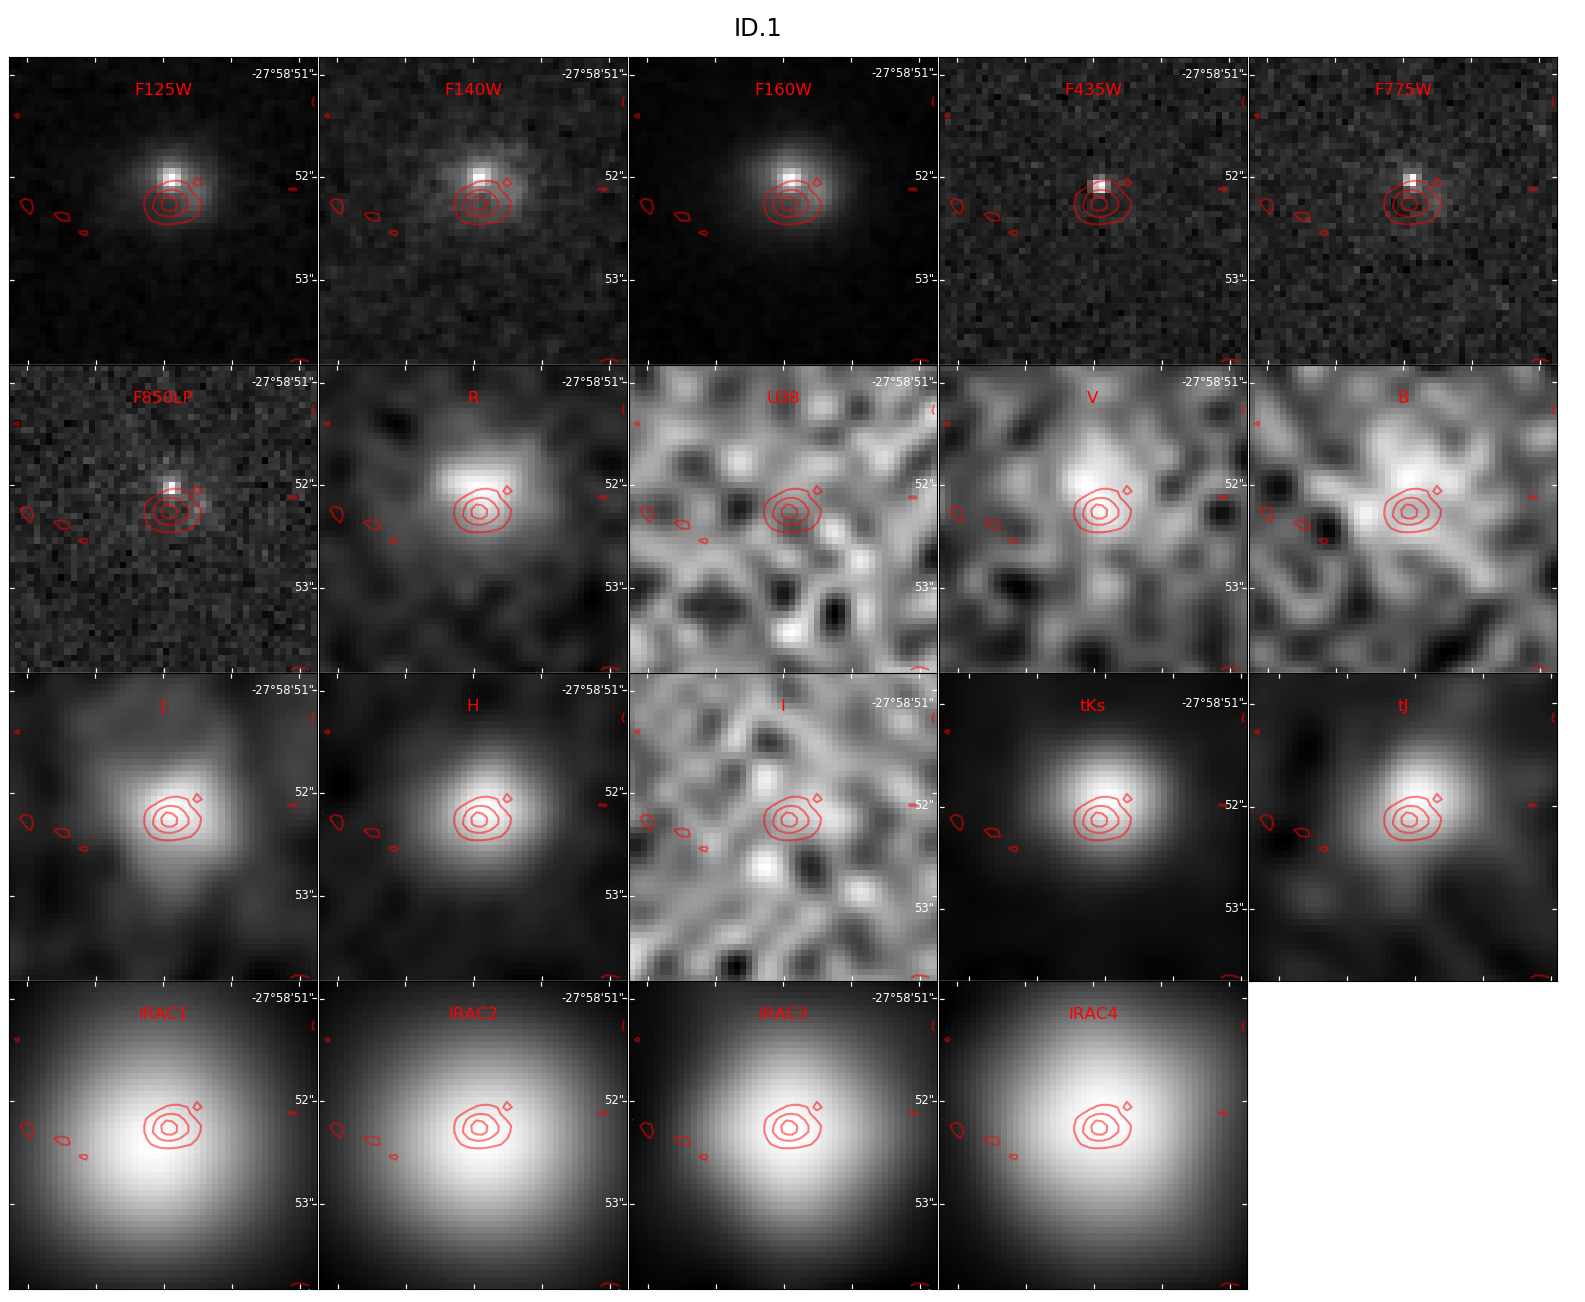
\includegraphics[width=160mm]{Matched/ASPECS_Cutout_0.jpg}
\caption{ID.1. Red contours signify +2$\sigma$,4$\sigma$,6$\sigma$,and 8$\sigma$. The size of the cutouts are 3x3 arcseconds.}
\label{fig:Match_One}
\end{figure}

\begin{figure}[tbp]
\centering 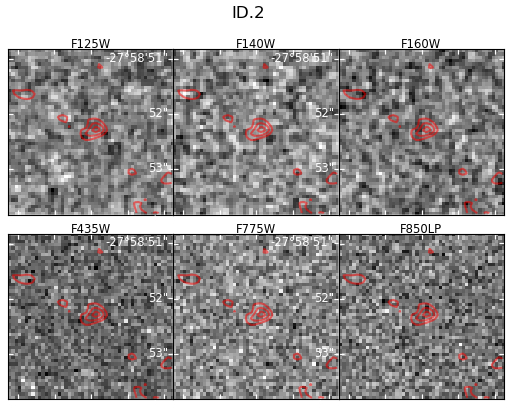
\includegraphics[width=160mm]{Matched/ASPECS_Cutout_1.jpg}
\caption{ID.2. Same contours and cutout size as for \ref{fig:Match_One}.}
\label{fig:Match_Two}
\end{figure}


\begin{figure}[tbp]
\centering 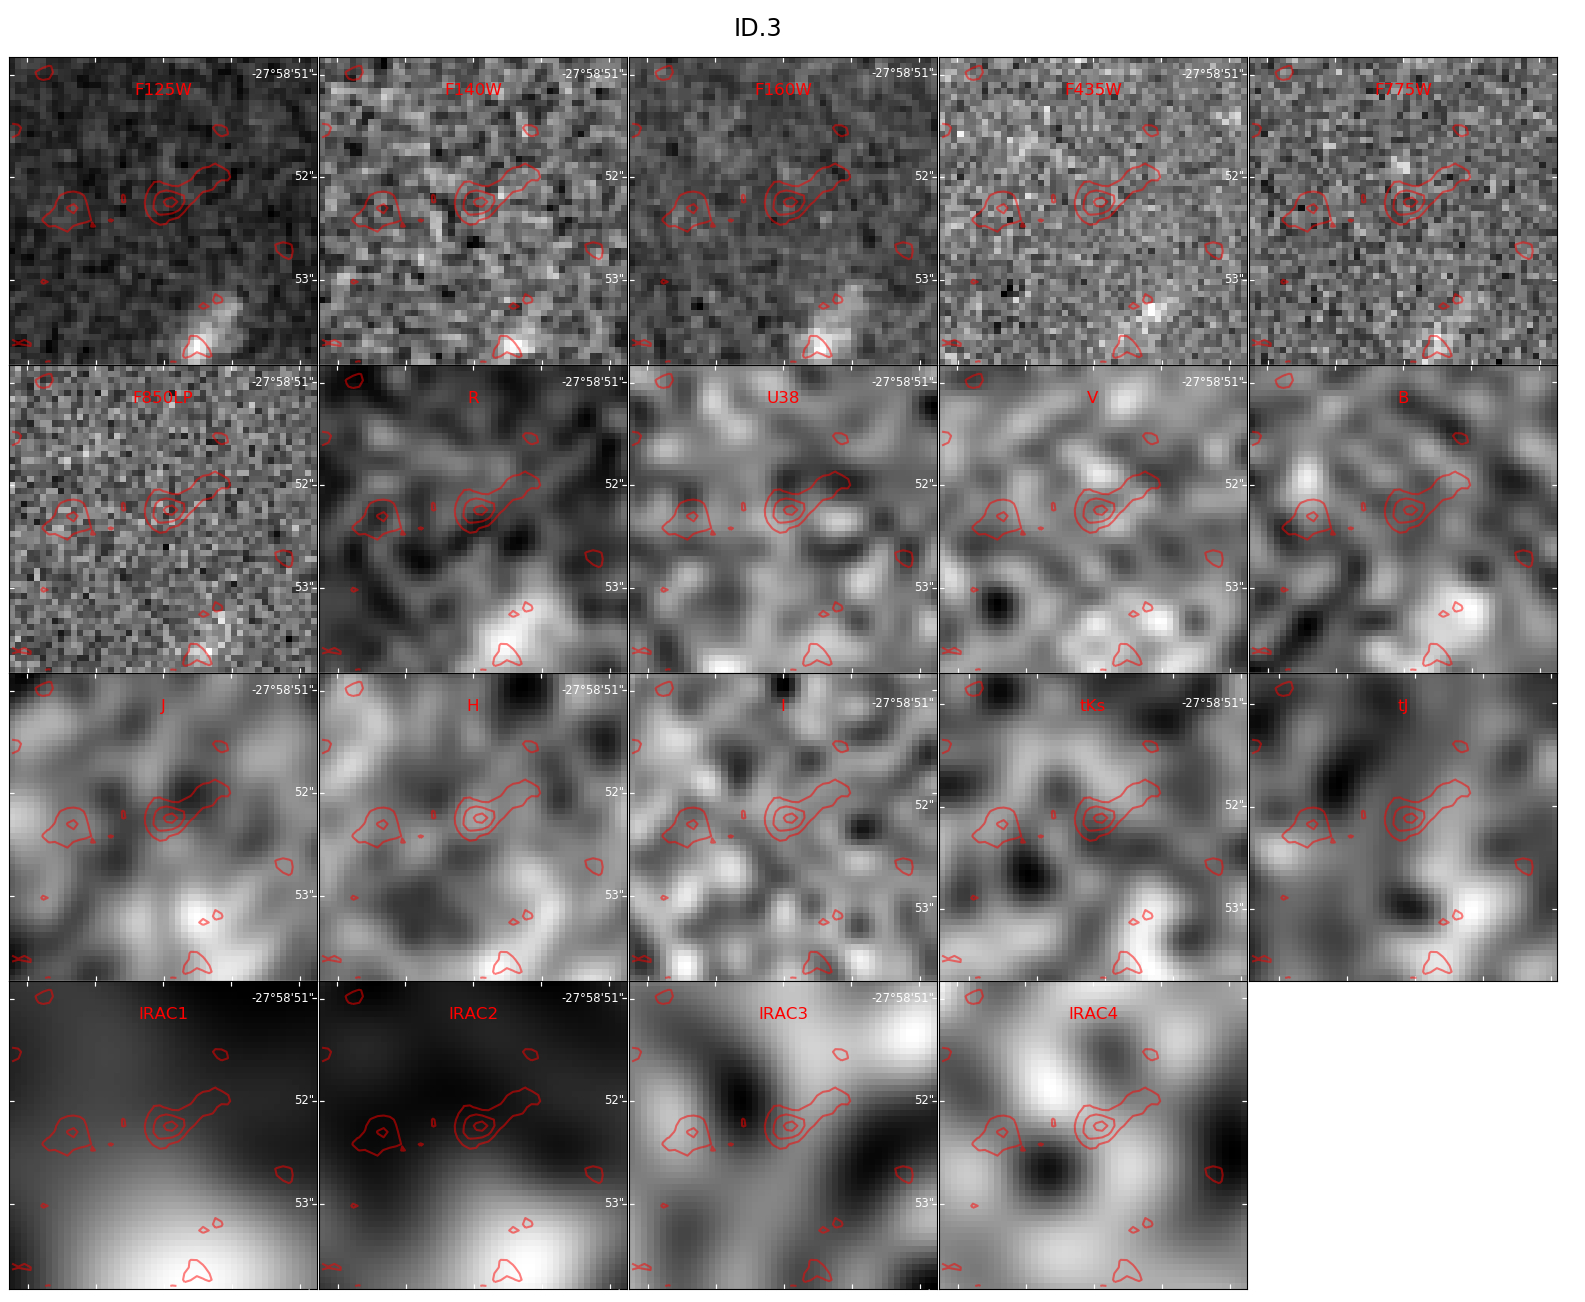
\includegraphics[width=160mm]{Matched/ASPECS_Cutout_2.jpg}
\caption{ID.3. Same contours and cutout size as for \ref{fig:Match_One}.}
\label{fig:Match_Three}
\end{figure}

\begin{figure}[tbp]
\centering 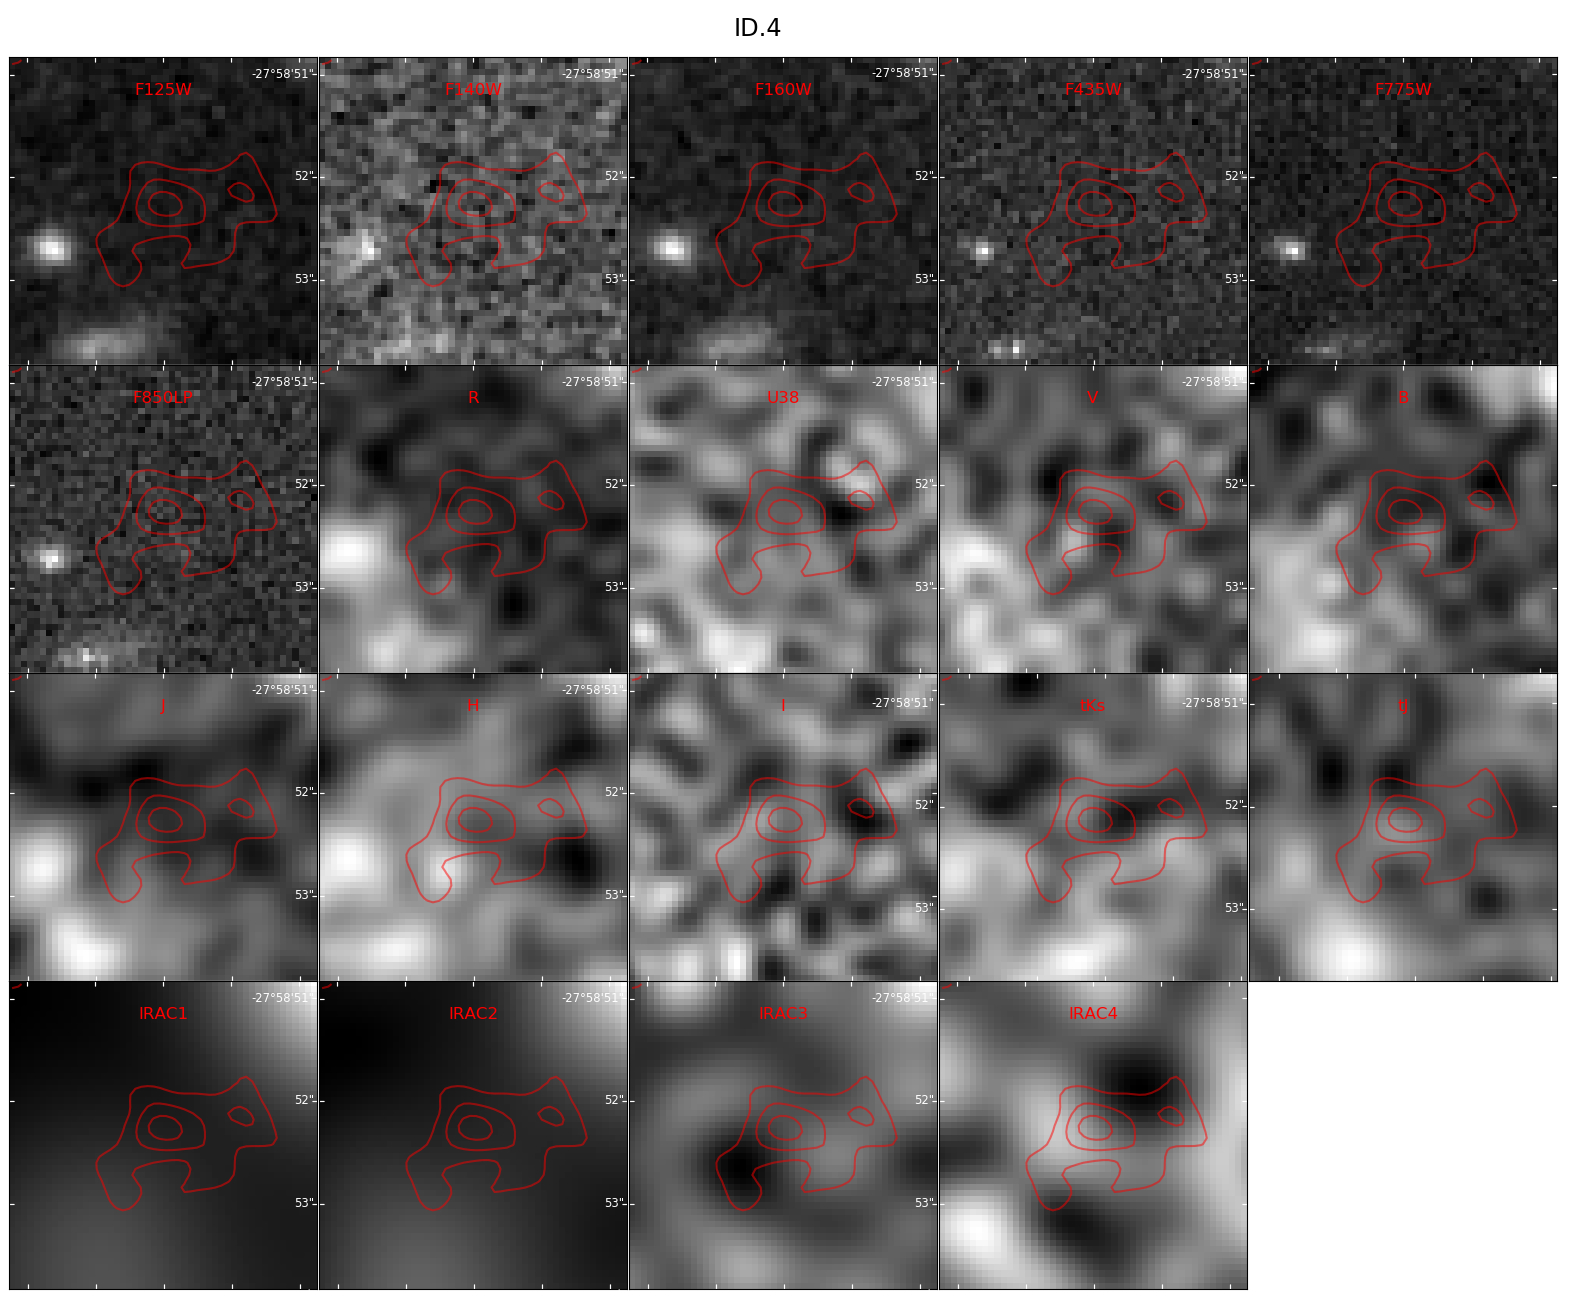
\includegraphics[width=160mm]{Matched/ASPECS_Cutout_3.jpg}
\caption{ID.4. Same contours and cutout size as for \ref{fig:Match_One}.}
\label{fig:Match_Three}
\end{figure}

\begin{figure}[tbp]
\centering 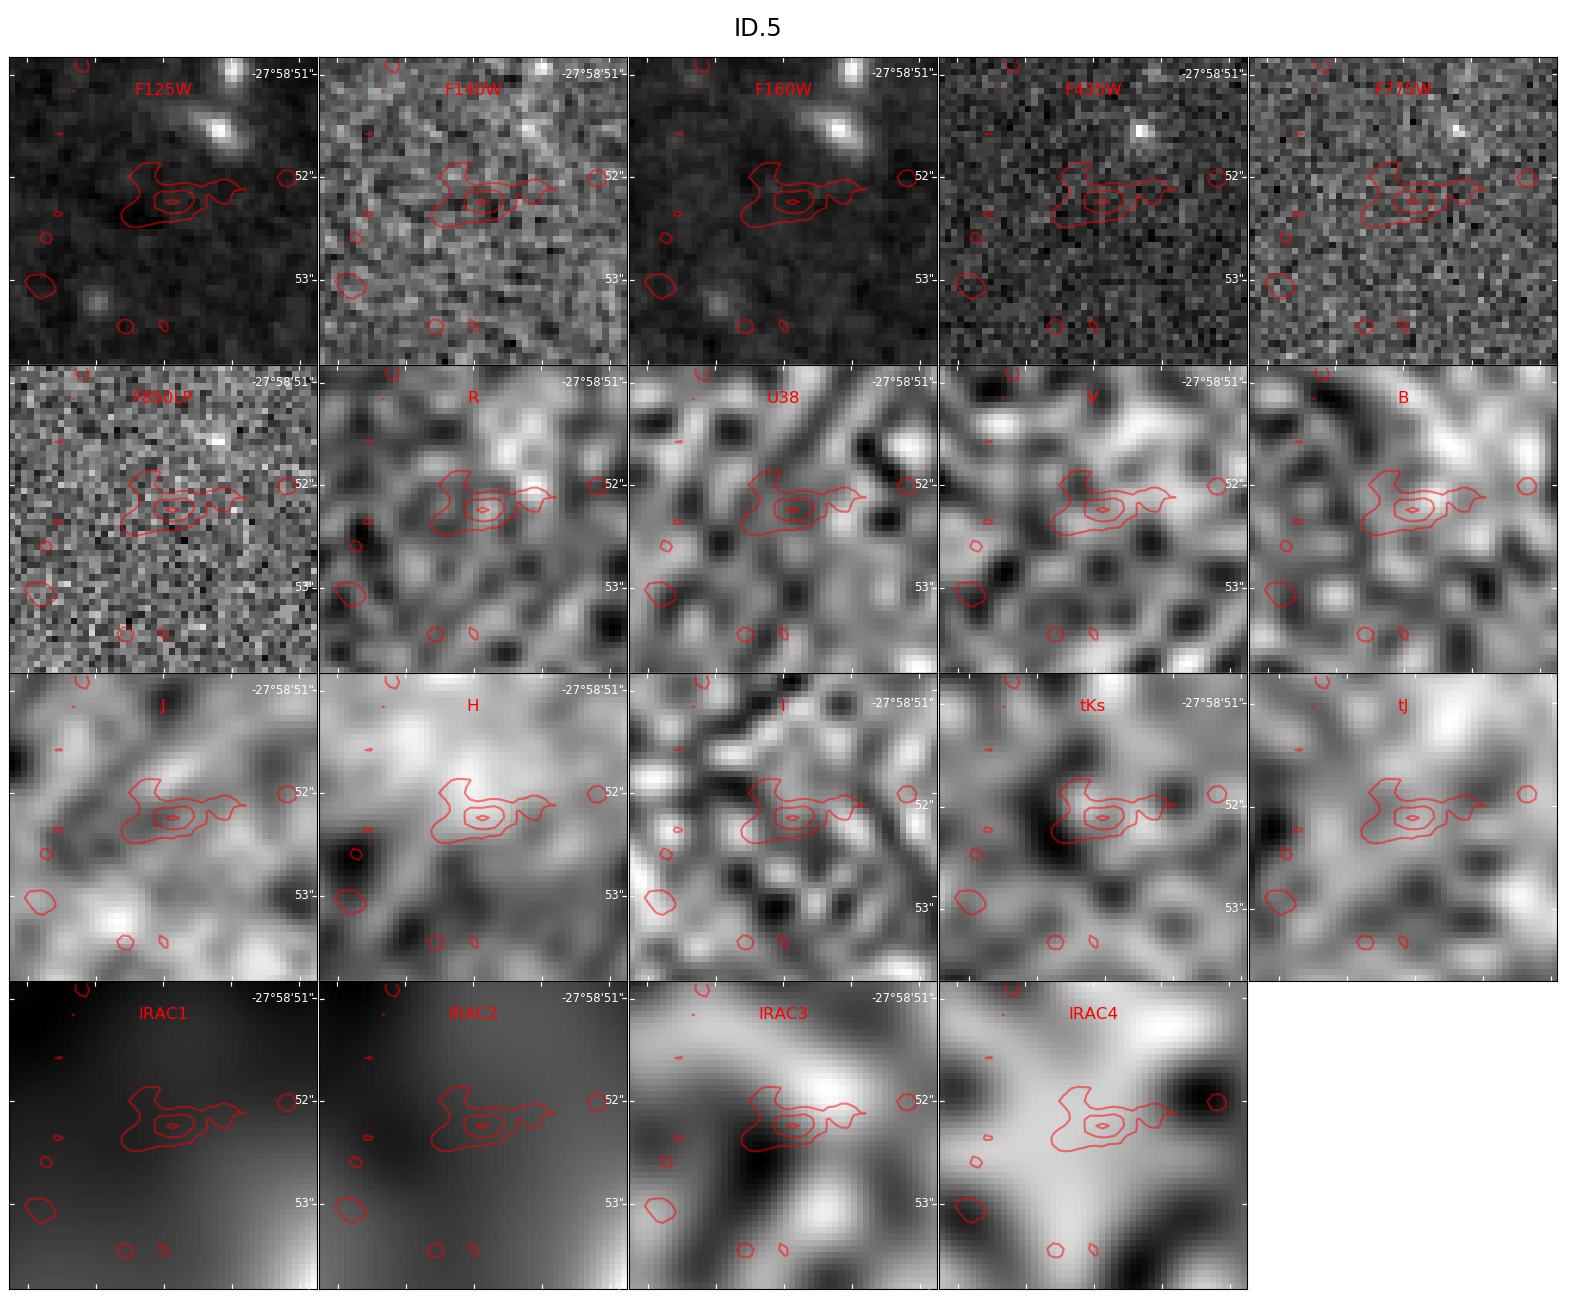
\includegraphics[width=160mm]{Matched/ASPECS_Cutout_4.jpg}
\caption{ID.5. Same contours and cutout size as for \ref{fig:Match_One}.}
\label{fig:Match_Four}
\end{figure}

\begin{figure}[tbp]
\centering 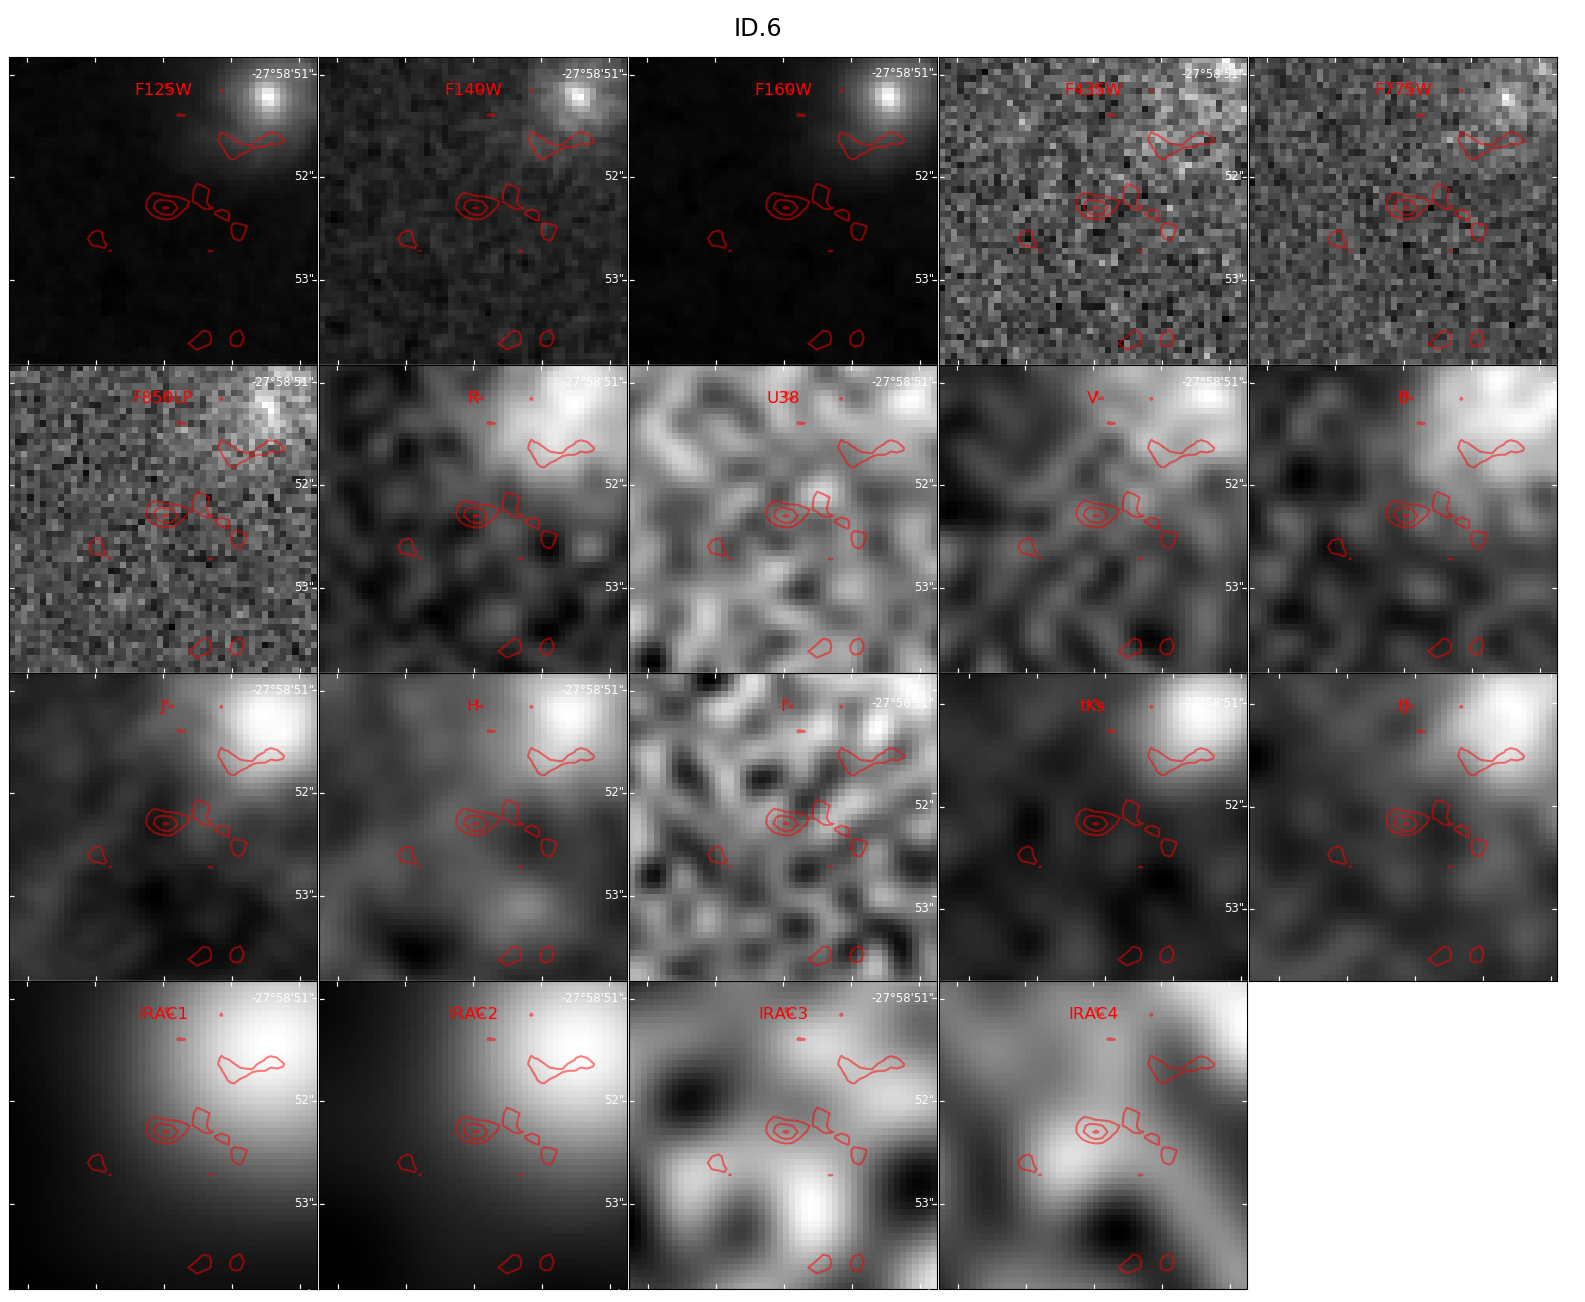
\includegraphics[width=160mm]{Matched/ASPECS_Cutout_5.jpg}
\caption{ID.6. Same contours and cutout size as for \ref{fig:Match_One}.}
\label{fig:Match_Five}
\end{figure}

\begin{figure}[tbp]
\centering 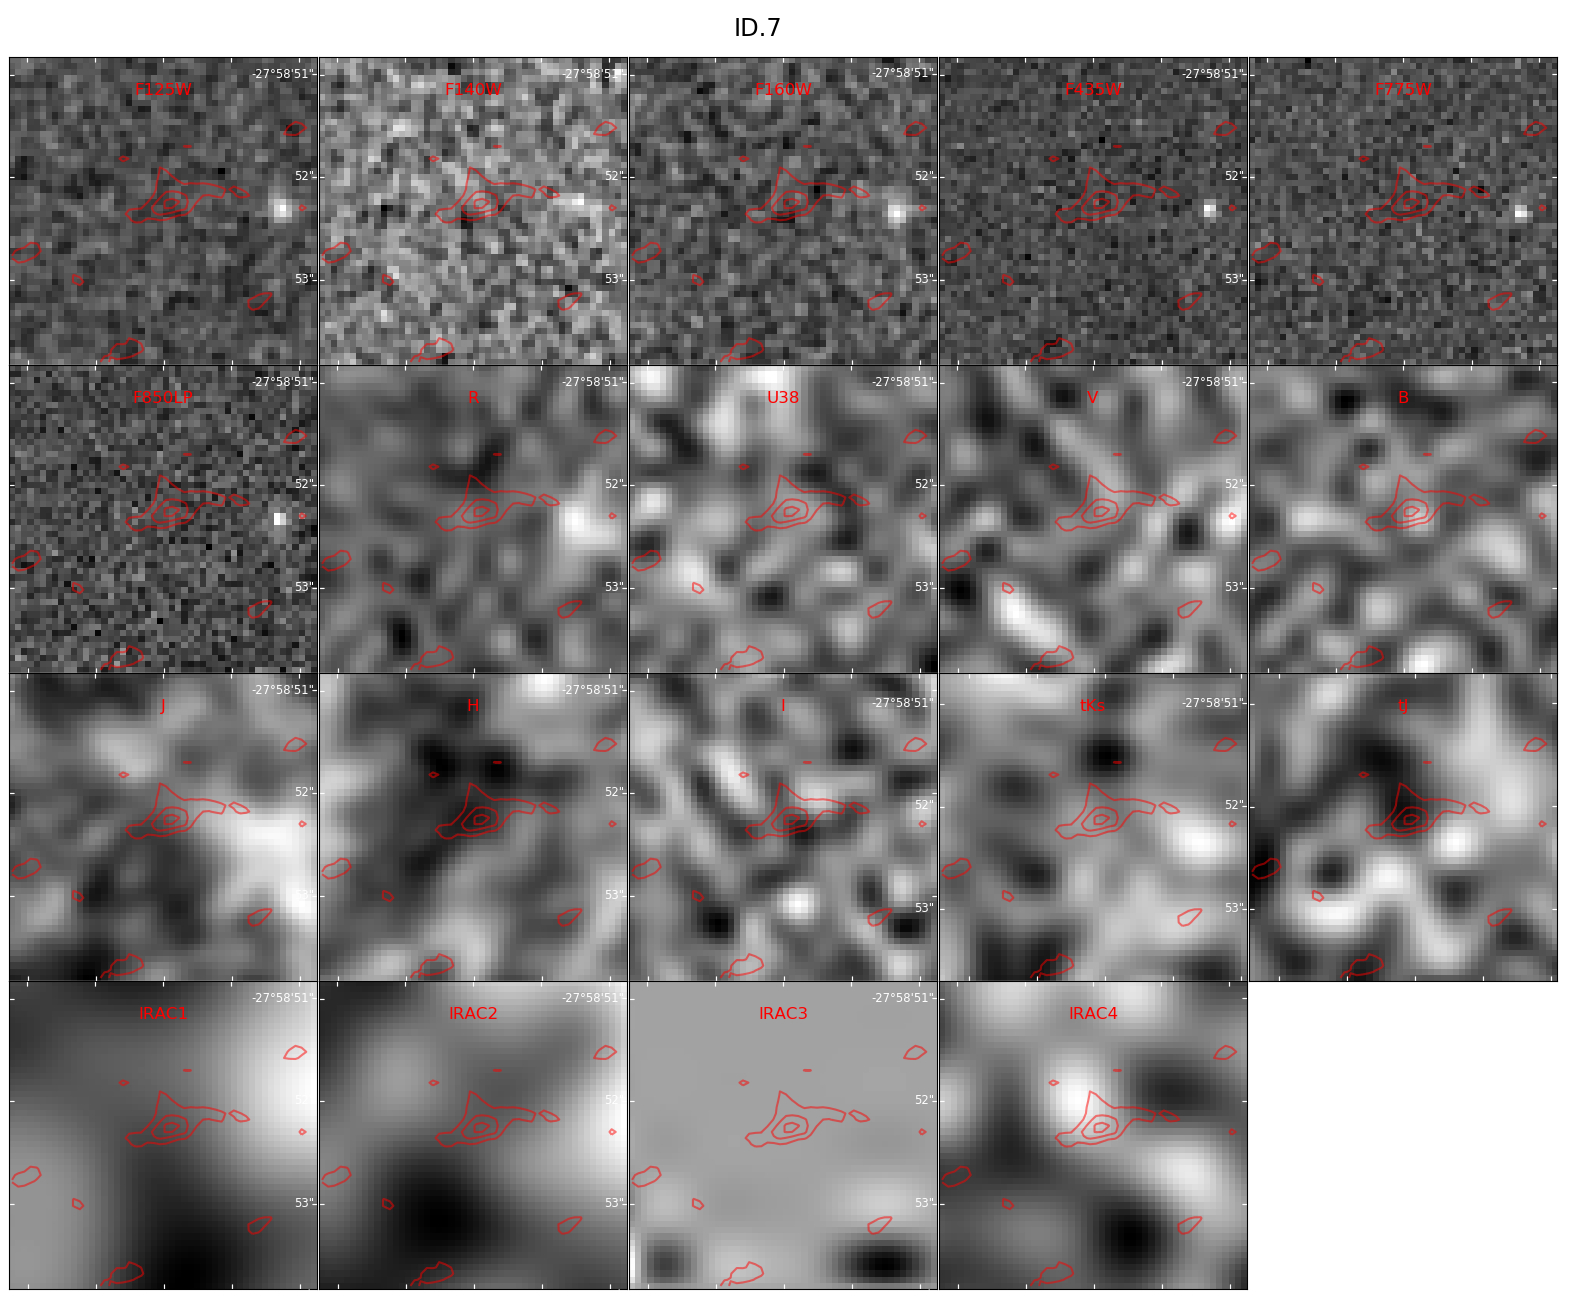
\includegraphics[width=160mm]{Matched/ASPECS_Cutout_6.jpg}
\caption{ID.7. Same contours and cutout size as for \ref{fig:Match_One}.}
\label{fig:Match_Three}
\end{figure}

\begin{figure}[tbp]
\centering 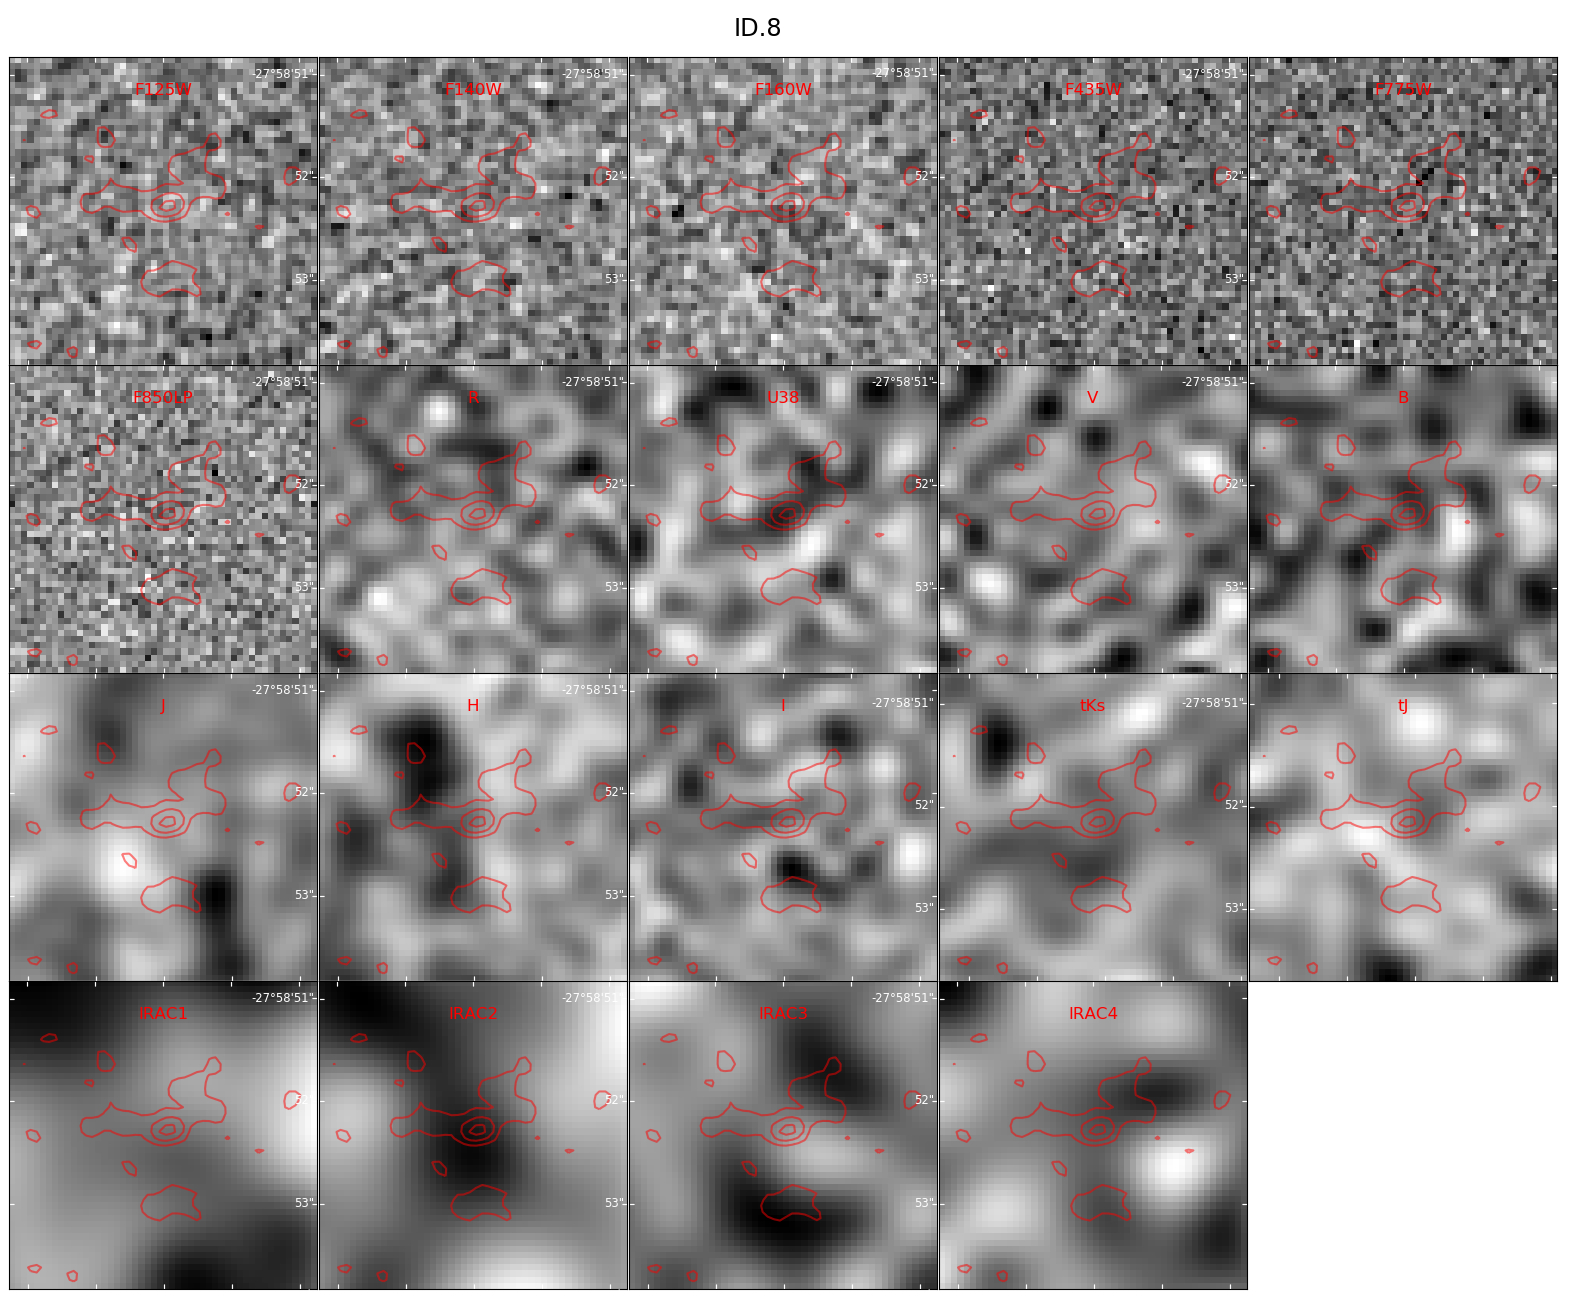
\includegraphics[width=160mm]{Matched/ASPECS_Cutout_7.jpg}
\caption{ID.8. Same contours and cutout size as for \ref{fig:Match_One}.}
\label{fig:Match_Three}
\end{figure}

\begin{figure}[tbp]
\centering 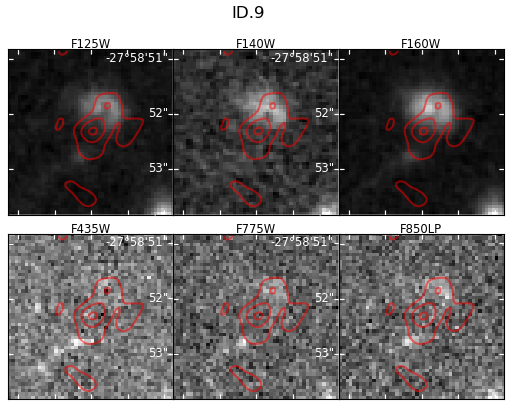
\includegraphics[width=160mm]{Matched/ASPECS_Cutout_8.jpg}
\caption{ID.9. Same contours and cutout size as for \ref{fig:Match_One}.}
\label{fig:Match_Three}
\end{figure}

\begin{figure}[tbp]
\centering 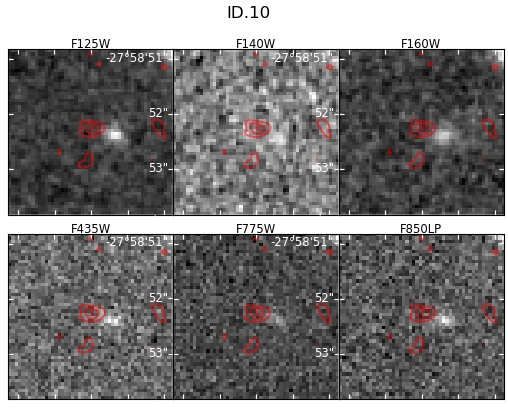
\includegraphics[width=160mm]{Matched/ASPECS_Cutout_9.jpg}
\caption{ID.10. Same contours and cutout size as for \ref{fig:Match_One}.}
\label{fig:Match_Three}
\end{figure}


\begin{figure}[tbp]
\centering 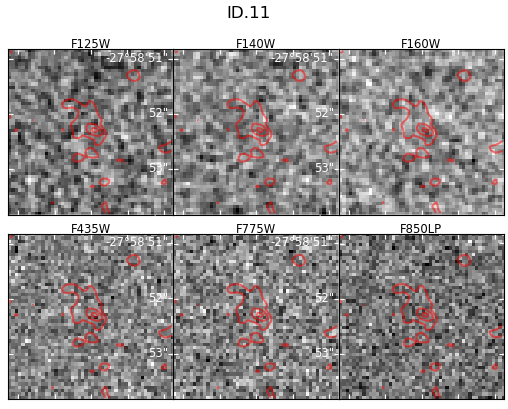
\includegraphics[width=160mm]{Matched/ASPECS_Cutout_10.jpg}
\caption{ID.11. Same contours and cutout size as for \ref{fig:Match_One}.}
\label{fig:Match_Three}
\end{figure}

\begin{figure}[tbp]
\centering 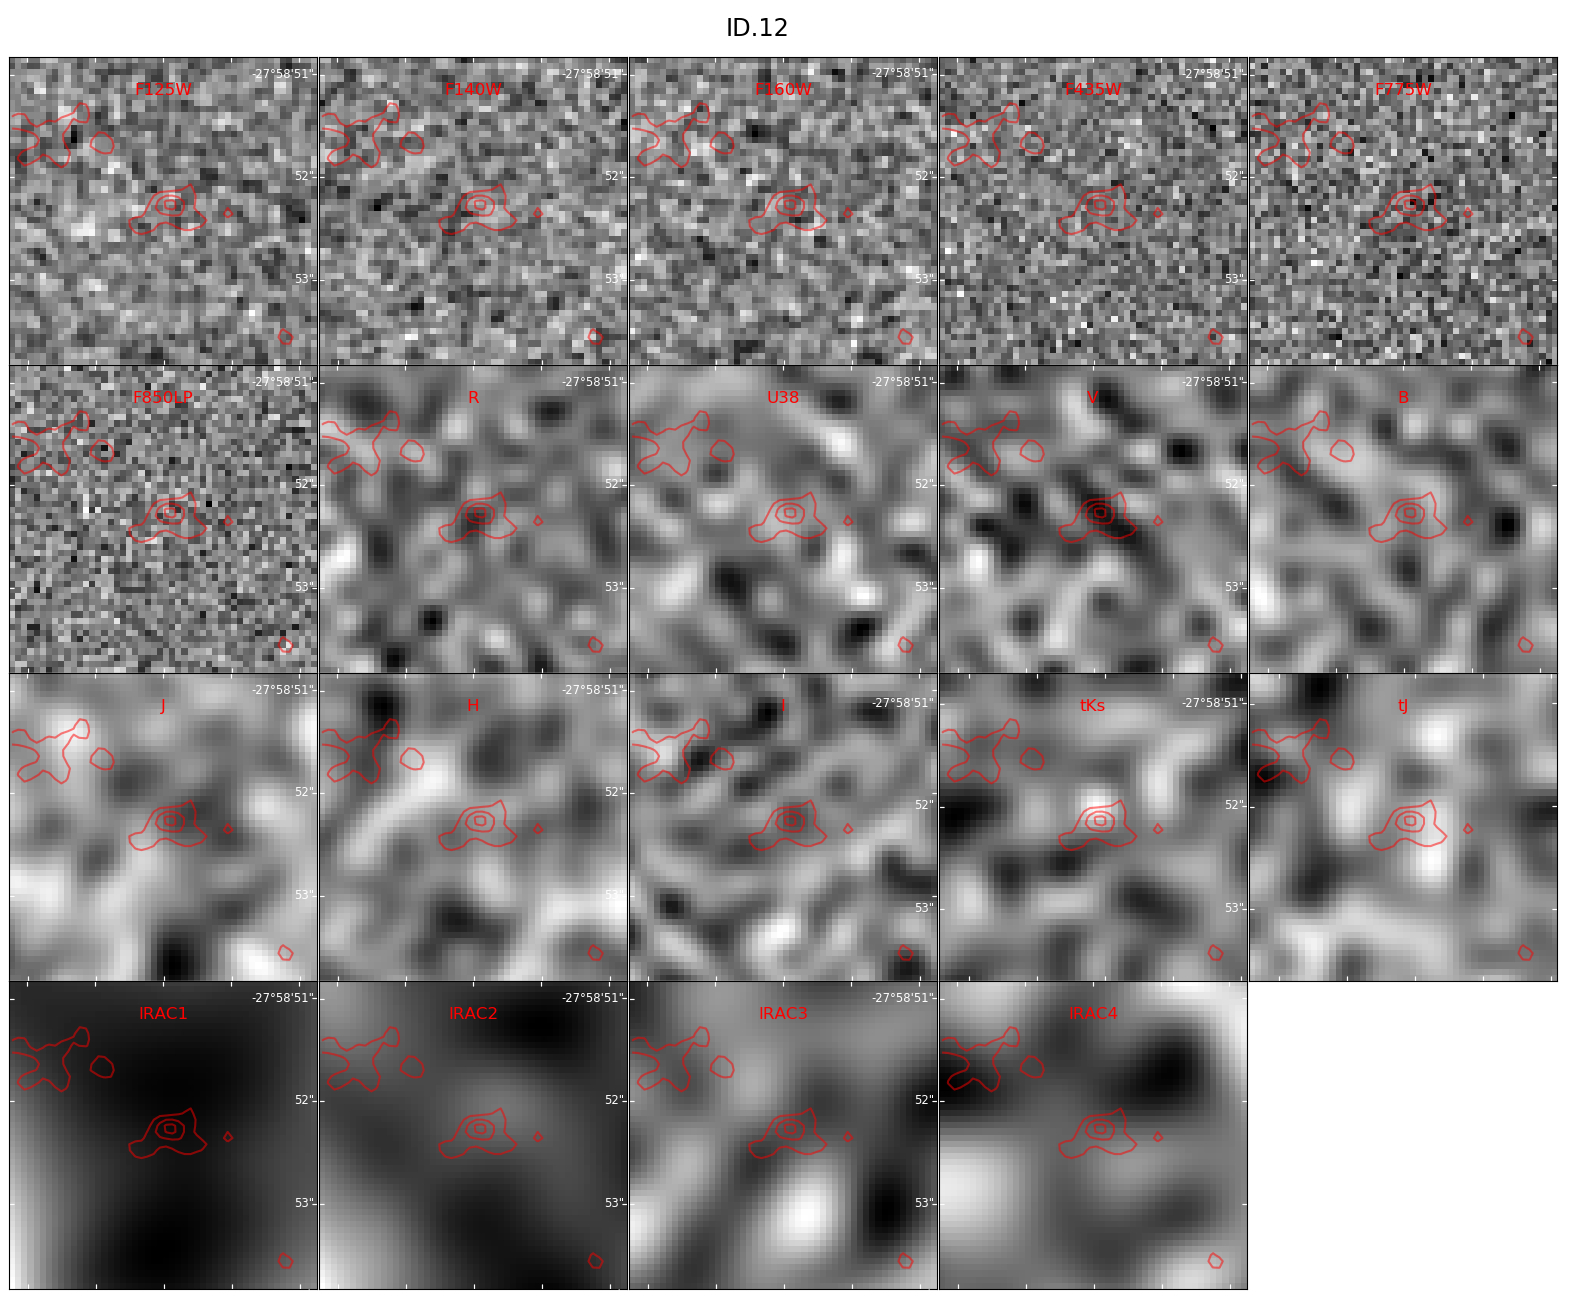
\includegraphics[width=160mm]{Matched/ASPECS_Cutout_11.jpg}
\caption{ID.12. Same contours and cutout size as for \ref{fig:Match_One}.}
\label{fig:Match_Three}
\end{figure}

\begin{figure}[tbp]
\centering 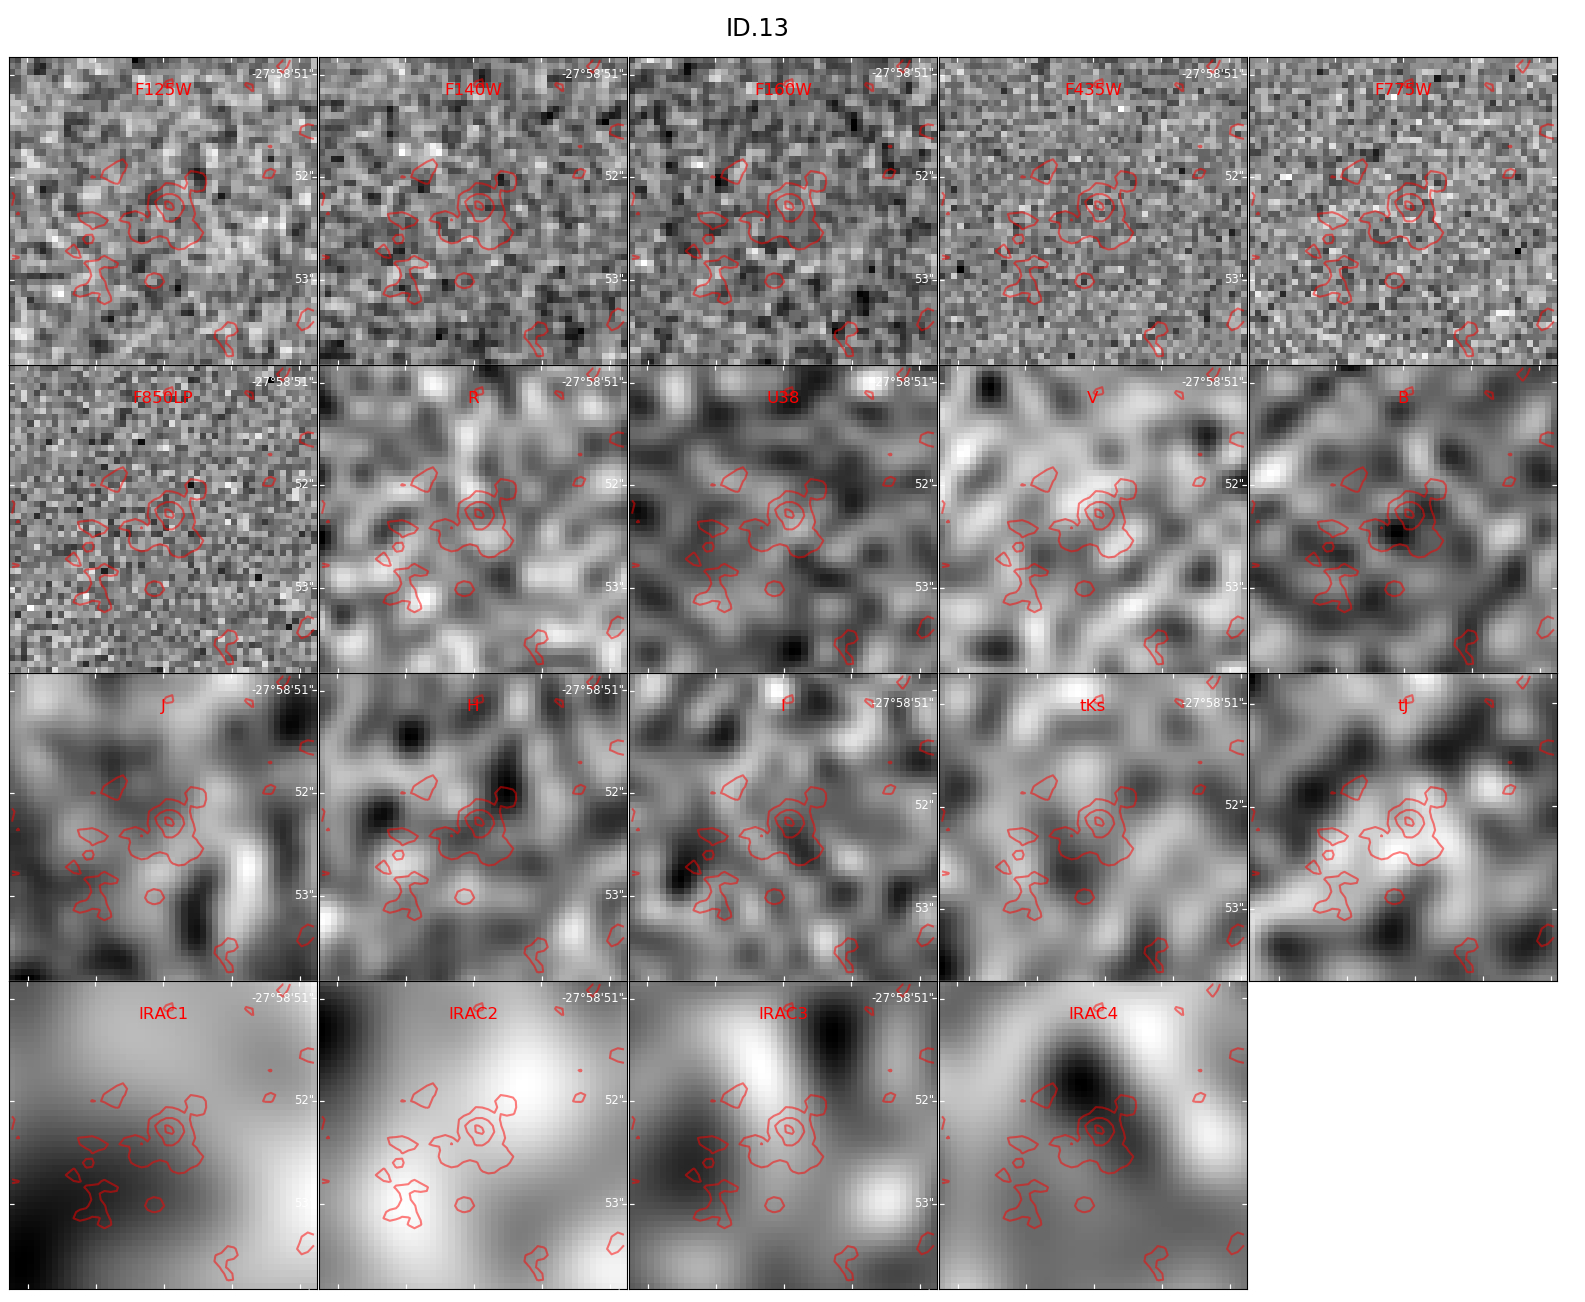
\includegraphics[width=160mm]{Matched/ASPECS_Cutout_12.jpg}
\caption{ID.13. Same contours and cutout size as for \ref{fig:Match_One}.}
\label{fig:Match_Three}
\end{figure}

\begin{figure}[tbp]
\centering 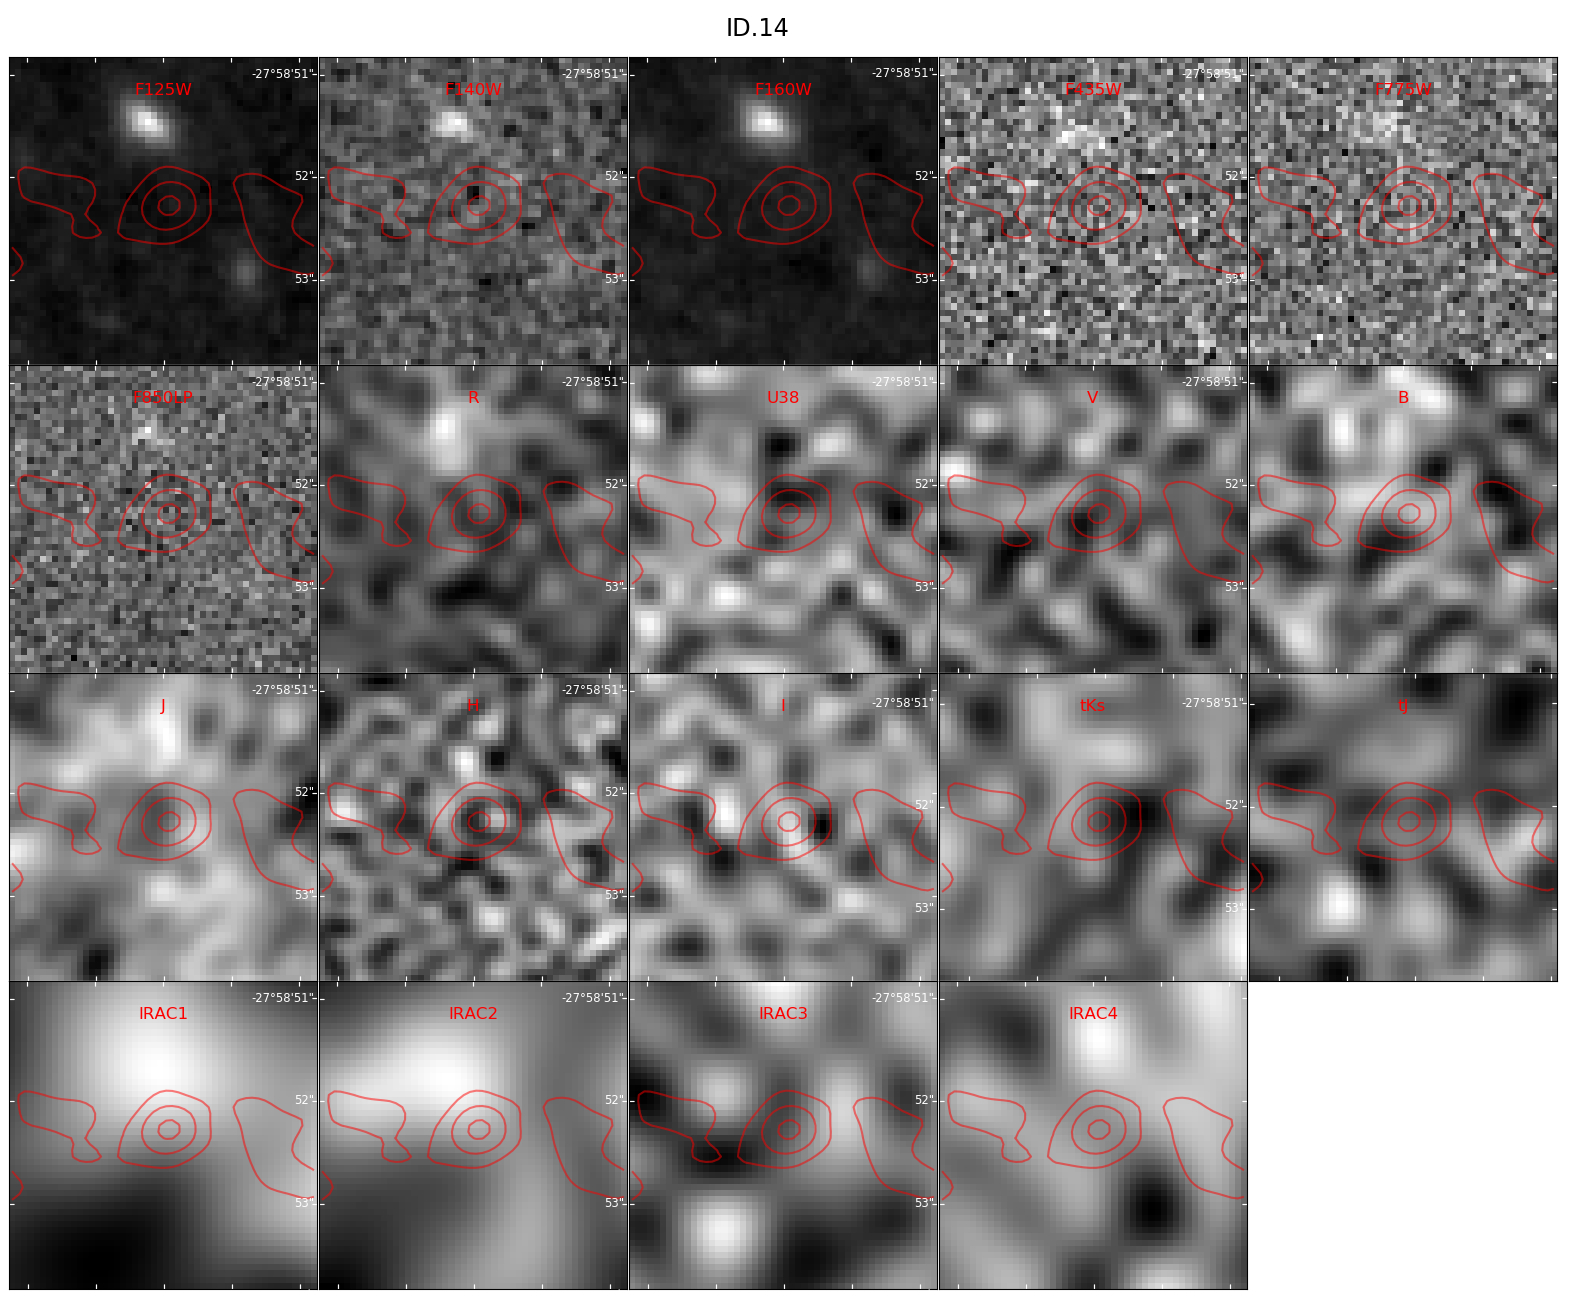
\includegraphics[width=160mm]{Matched/ASPECS_Cutout_13.jpg}
\caption{ID.14. Same contours and cutout size as for \ref{fig:Match_One}.}
\label{fig:Match_Three}
\end{figure}

\begin{figure}[tbp]
\centering 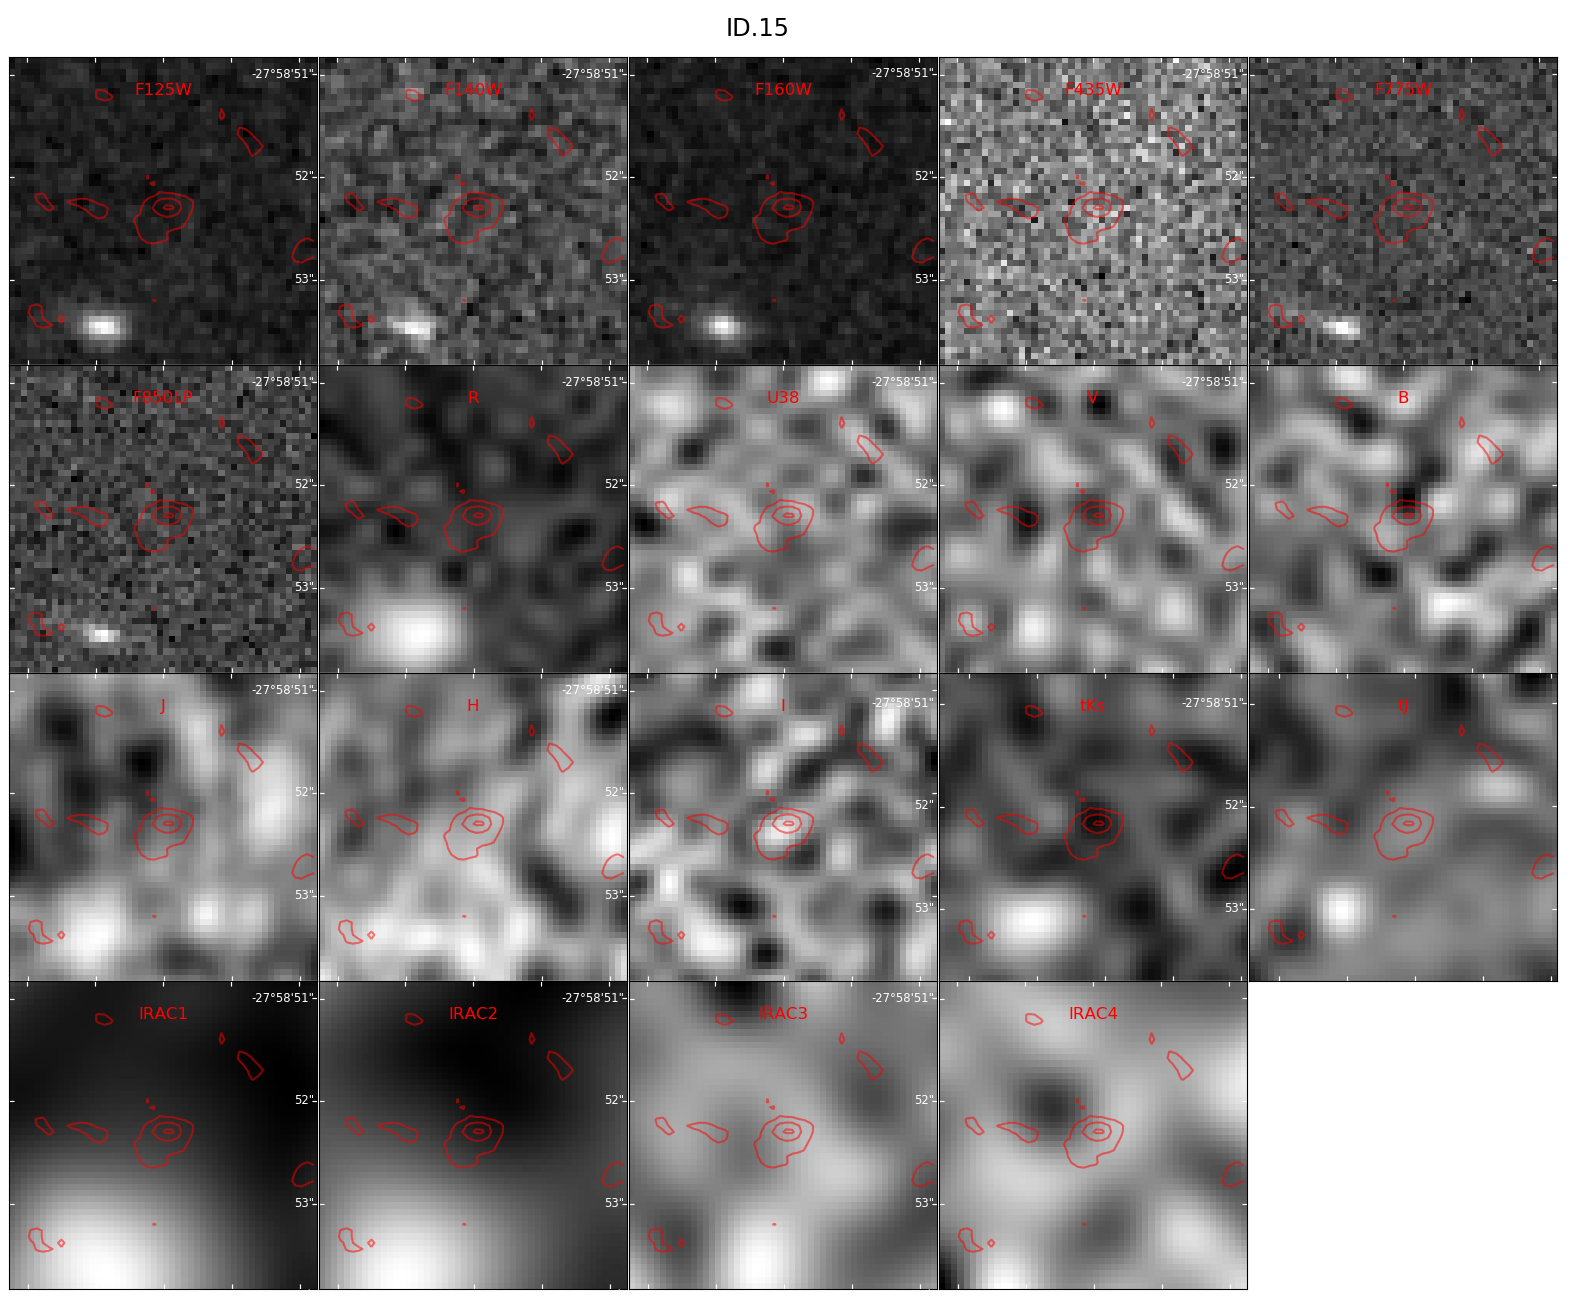
\includegraphics[width=160mm]{Matched/ASPECS_Cutout_14.jpg}
\caption{ID.15. Same contours and cutout size as for \ref{fig:Match_One}.}
\label{fig:Match_Three}
\end{figure}

\begin{figure}[tbp]
\centering 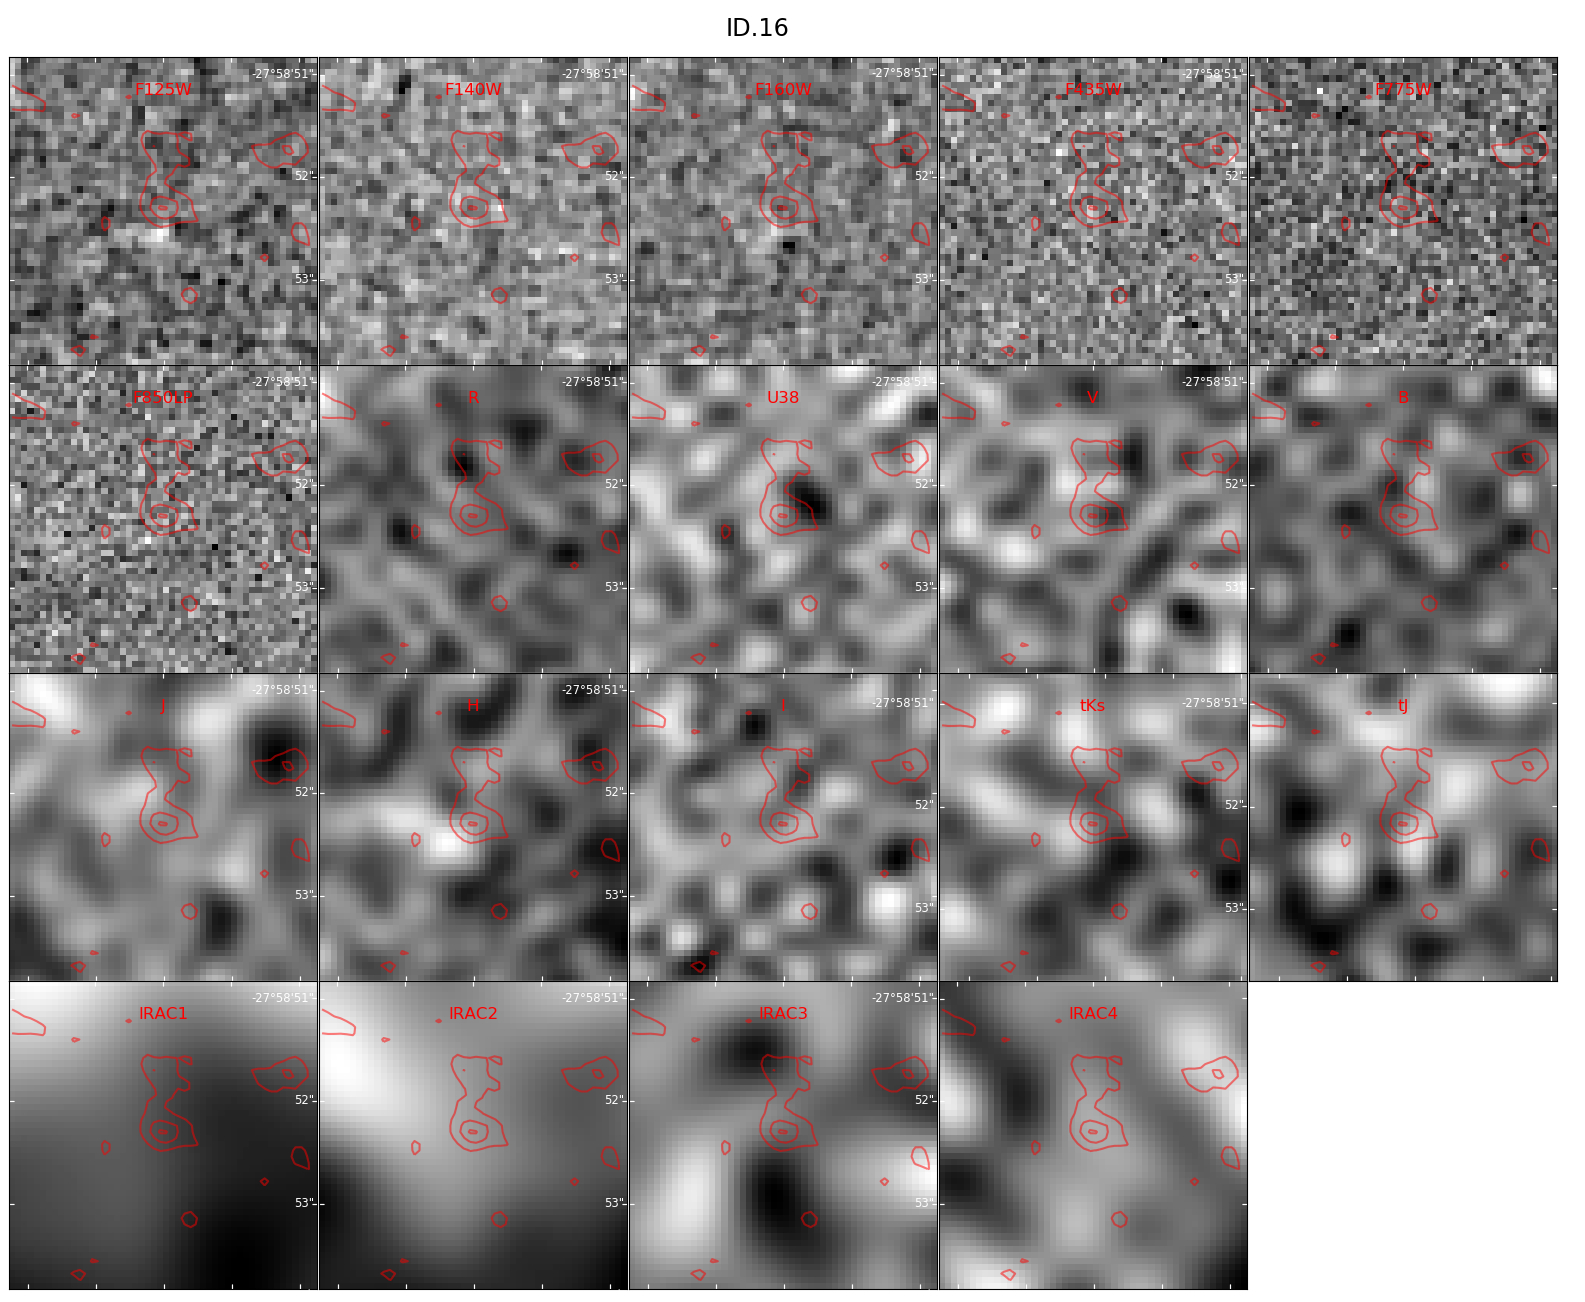
\includegraphics[width=160mm]{Matched/ASPECS_Cutout_15.jpg}
\caption{ID.16. Same contours and cutout size as for \ref{fig:Match_One}.}
\label{fig:Match_Three}
\end{figure}

\begin{figure}[tbp]
\centering 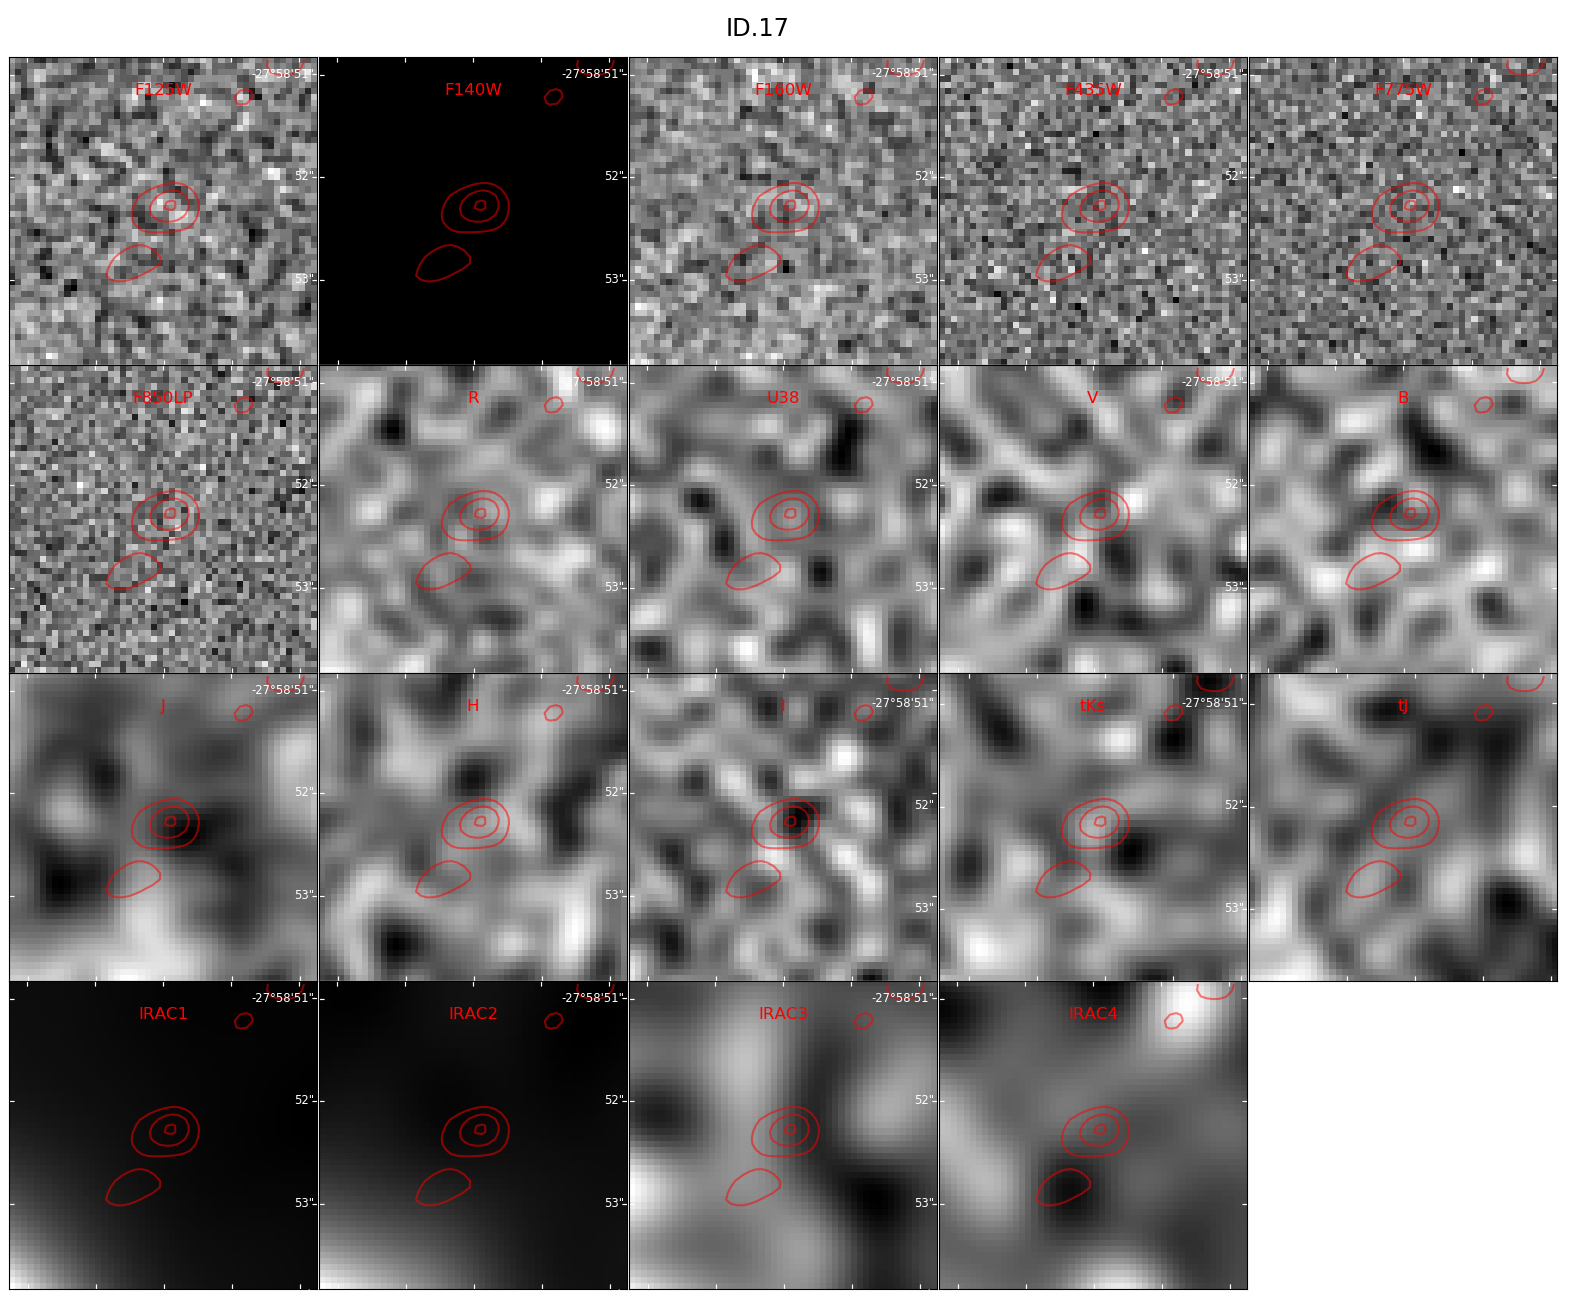
\includegraphics[width=160mm]{Matched/ASPECS_Cutout_16.jpg}
\caption{ID.17. Same contours and cutout size as for \ref{fig:Match_One}.}
\label{fig:Match_Three}
\end{figure}

\begin{figure}[tbp]
\centering 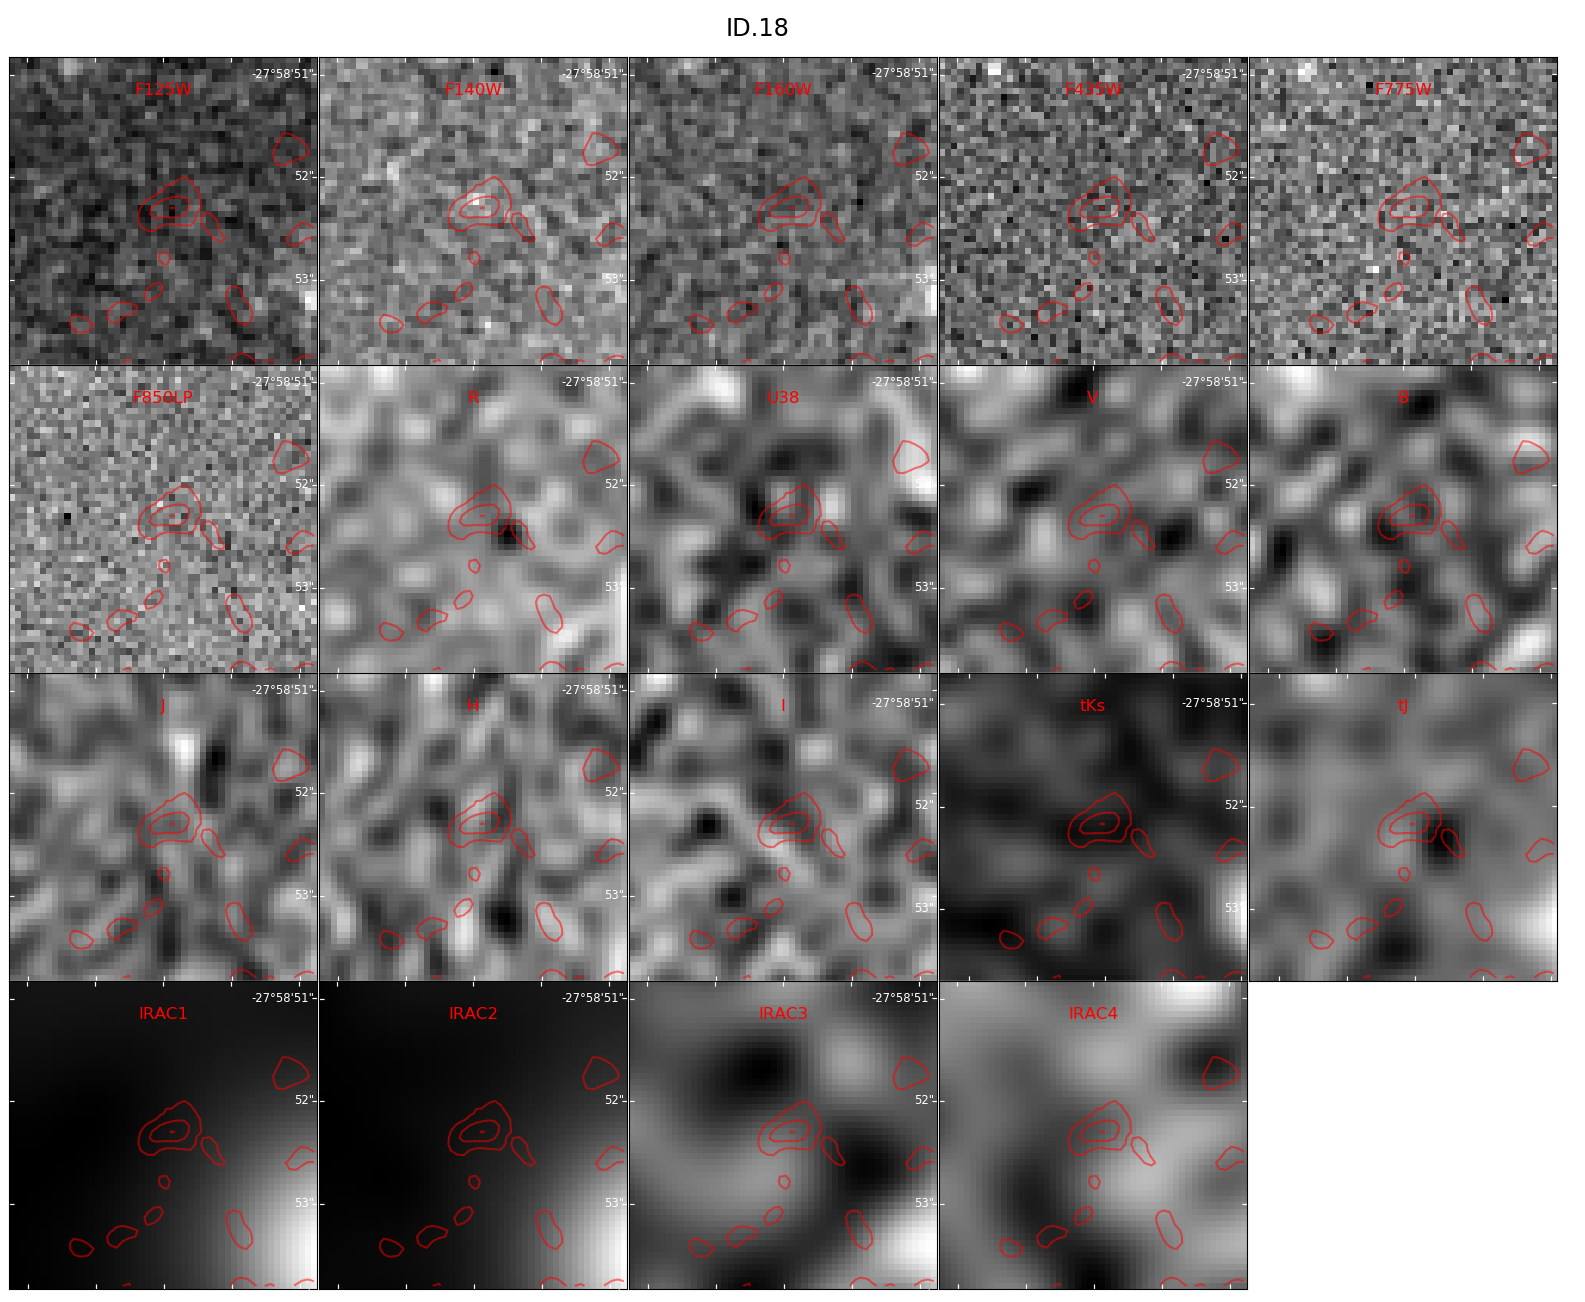
\includegraphics[width=160mm]{Matched/ASPECS_Cutout_17.jpg}
\caption{ID.18. Same contours and cutout size as for \ref{fig:Match_One}.}
\label{fig:Match_Three}
\end{figure}

\begin{figure}[tbp]
\centering 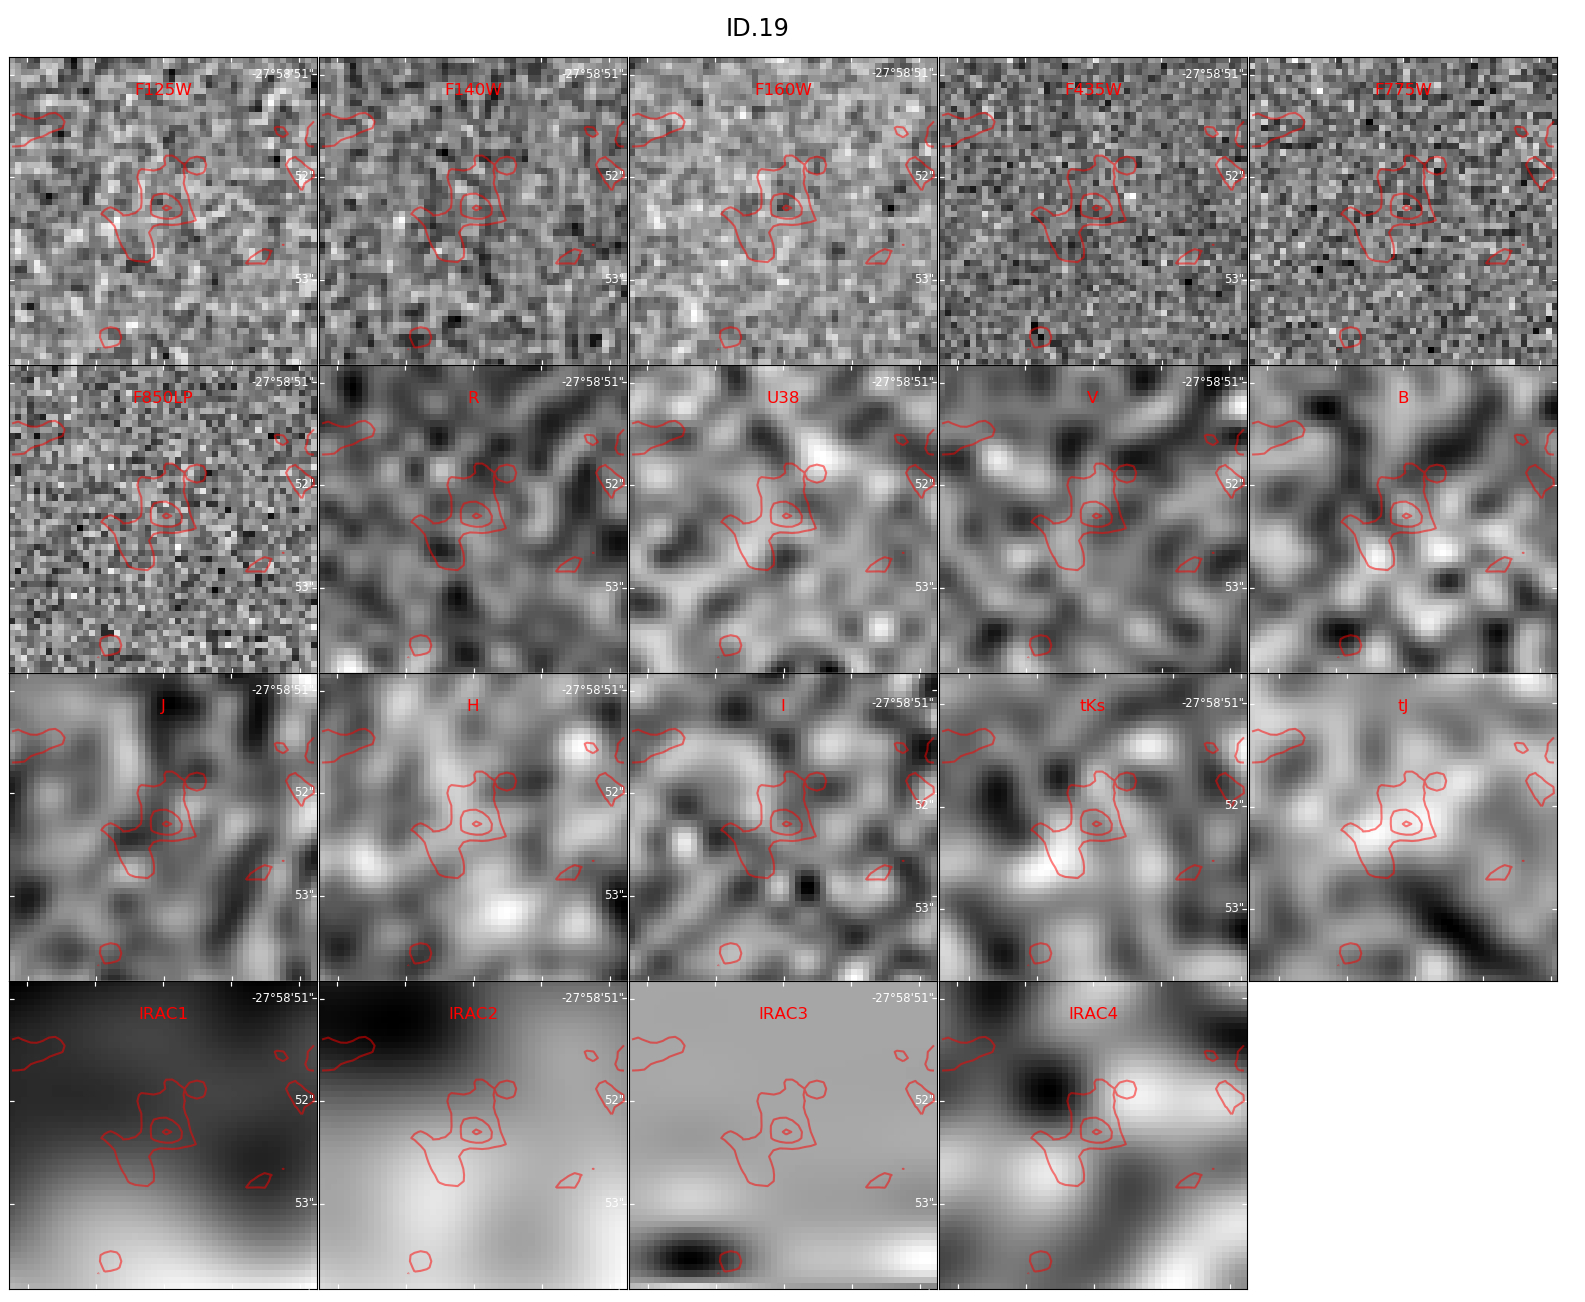
\includegraphics[width=160mm]{Matched/ASPECS_Cutout_18.jpg}
\caption{ID.19. Same contours and cutout size as for \ref{fig:Match_One}.}
\label{fig:Match_Three}
\end{figure}

\begin{figure}[tbp]
\centering 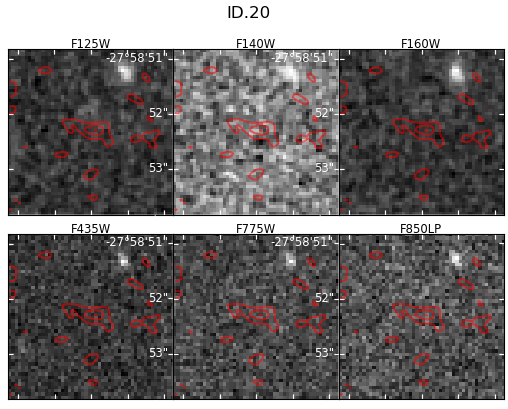
\includegraphics[width=160mm]{Matched/ASPECS_Cutout_19.jpg}
\caption{ID.20. Same contours and cutout size as for \ref{fig:Match_One}.}
\label{fig:Match_Three}
\end{figure}

\begin{figure}[tbp]
\centering 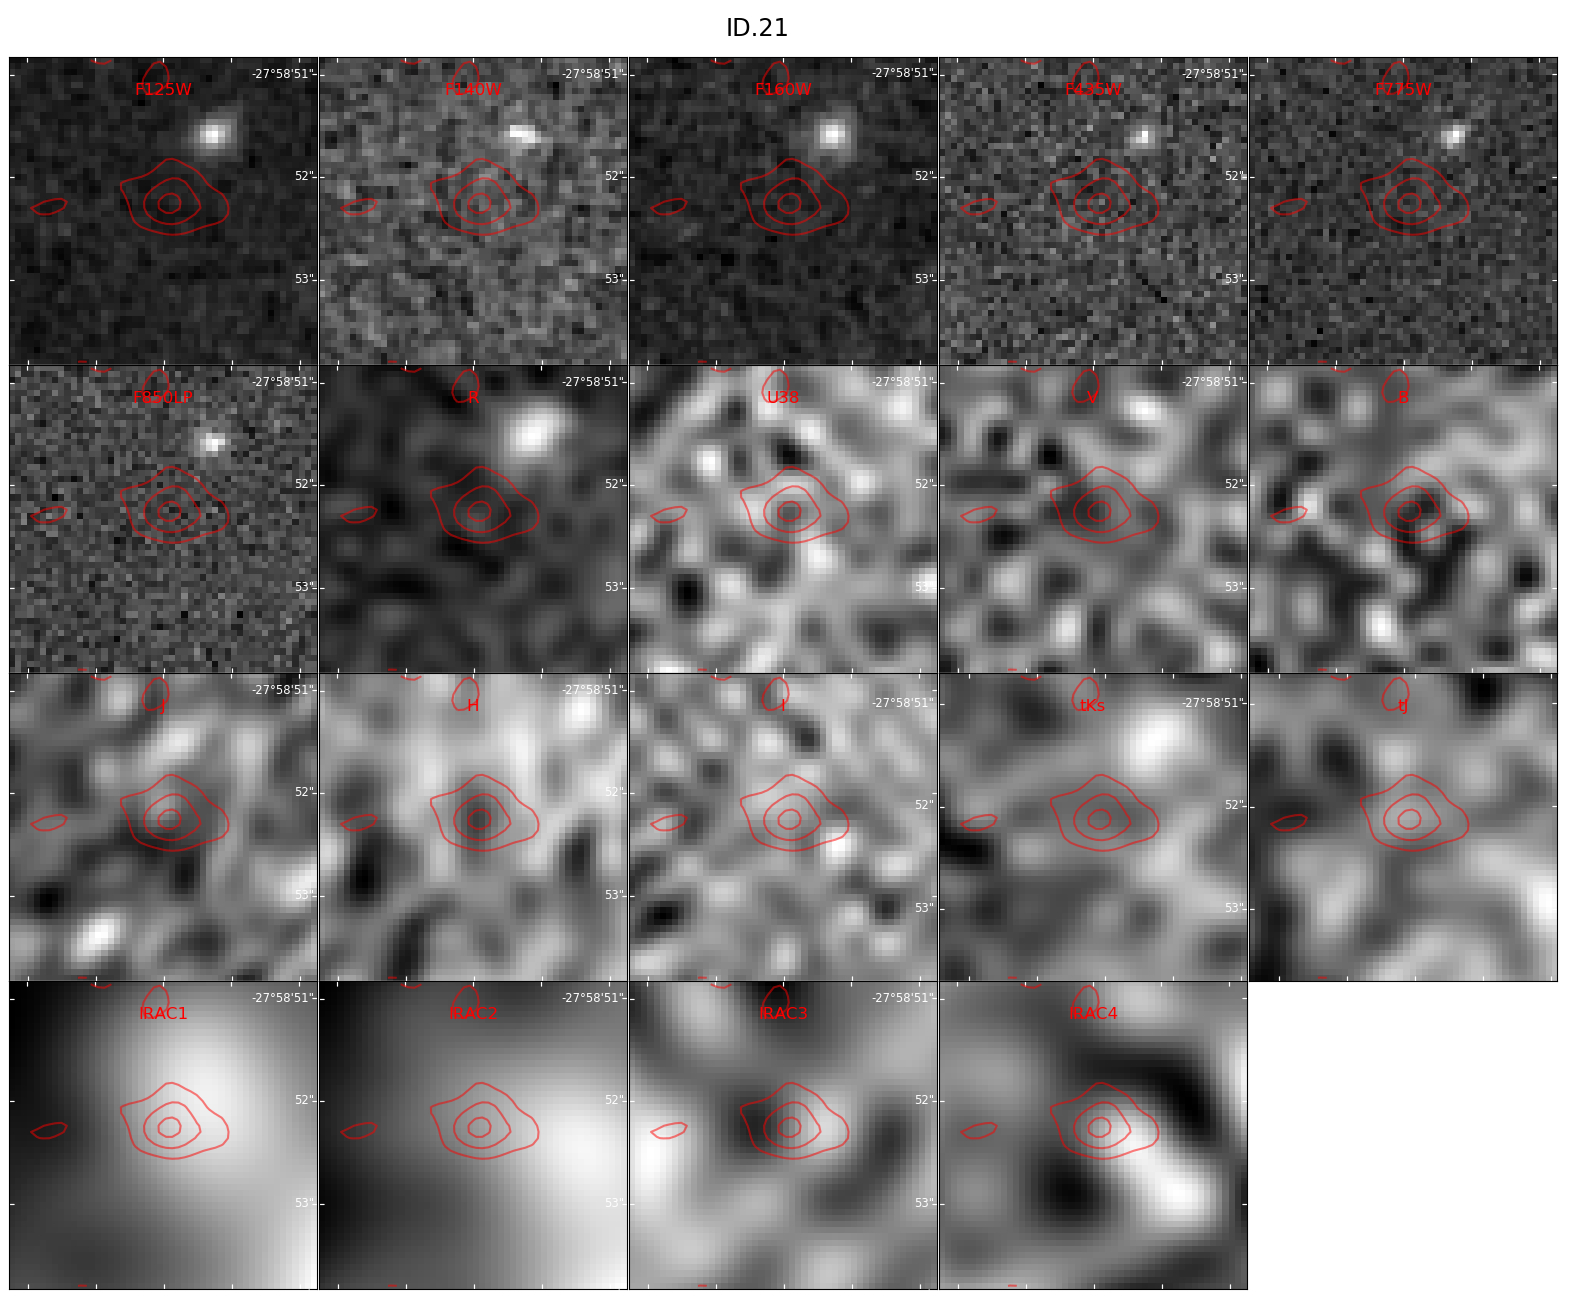
\includegraphics[width=160mm]{Matched/ASPECS_Cutout_20.jpg}
\caption{ID.21. Same contours and cutout size as for \ref{fig:Match_One}.}
\label{fig:Match_Three}
\end{figure}

\begin{figure}[tbp]
\centering 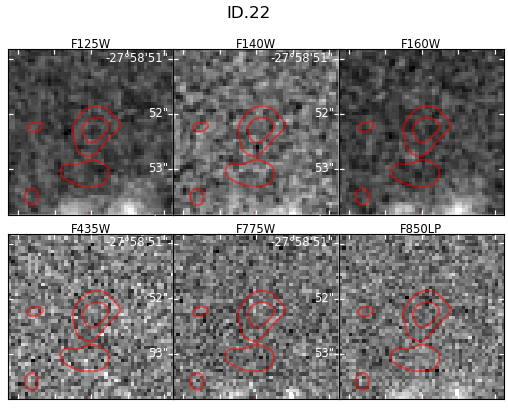
\includegraphics[width=160mm]{Matched/ASPECS_Cutout_21.jpg}
\caption{ID.22. Same contours and cutout size as for \ref{fig:Match_One}.}
\label{fig:Match_Three}
\end{figure}

\begin{figure}[tbp]
\centering 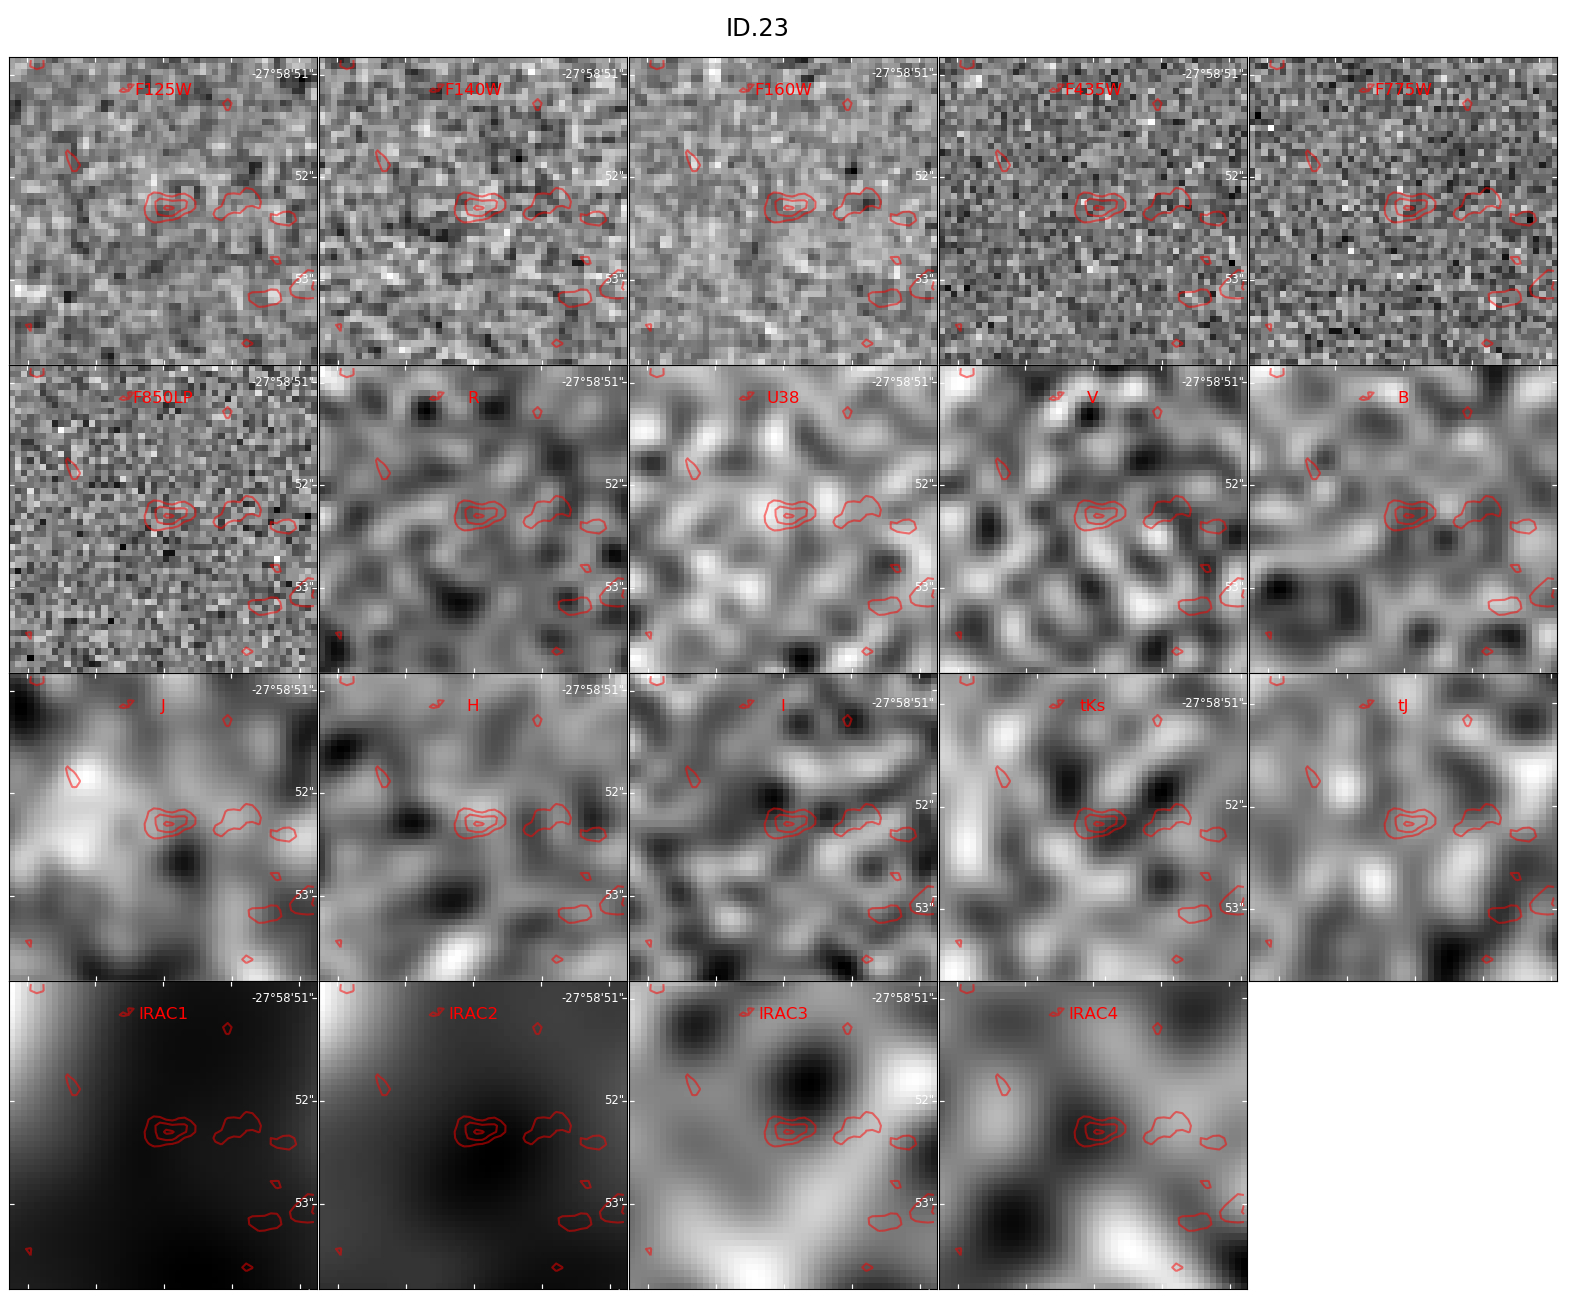
\includegraphics[width=160mm]{Matched/ASPECS_Cutout_22.jpg}
\caption{ID.23. Same contours and cutout size as for \ref{fig:Match_One}.}
\label{fig:Match_Three}
\end{figure}

\begin{figure}[tbp]
\centering 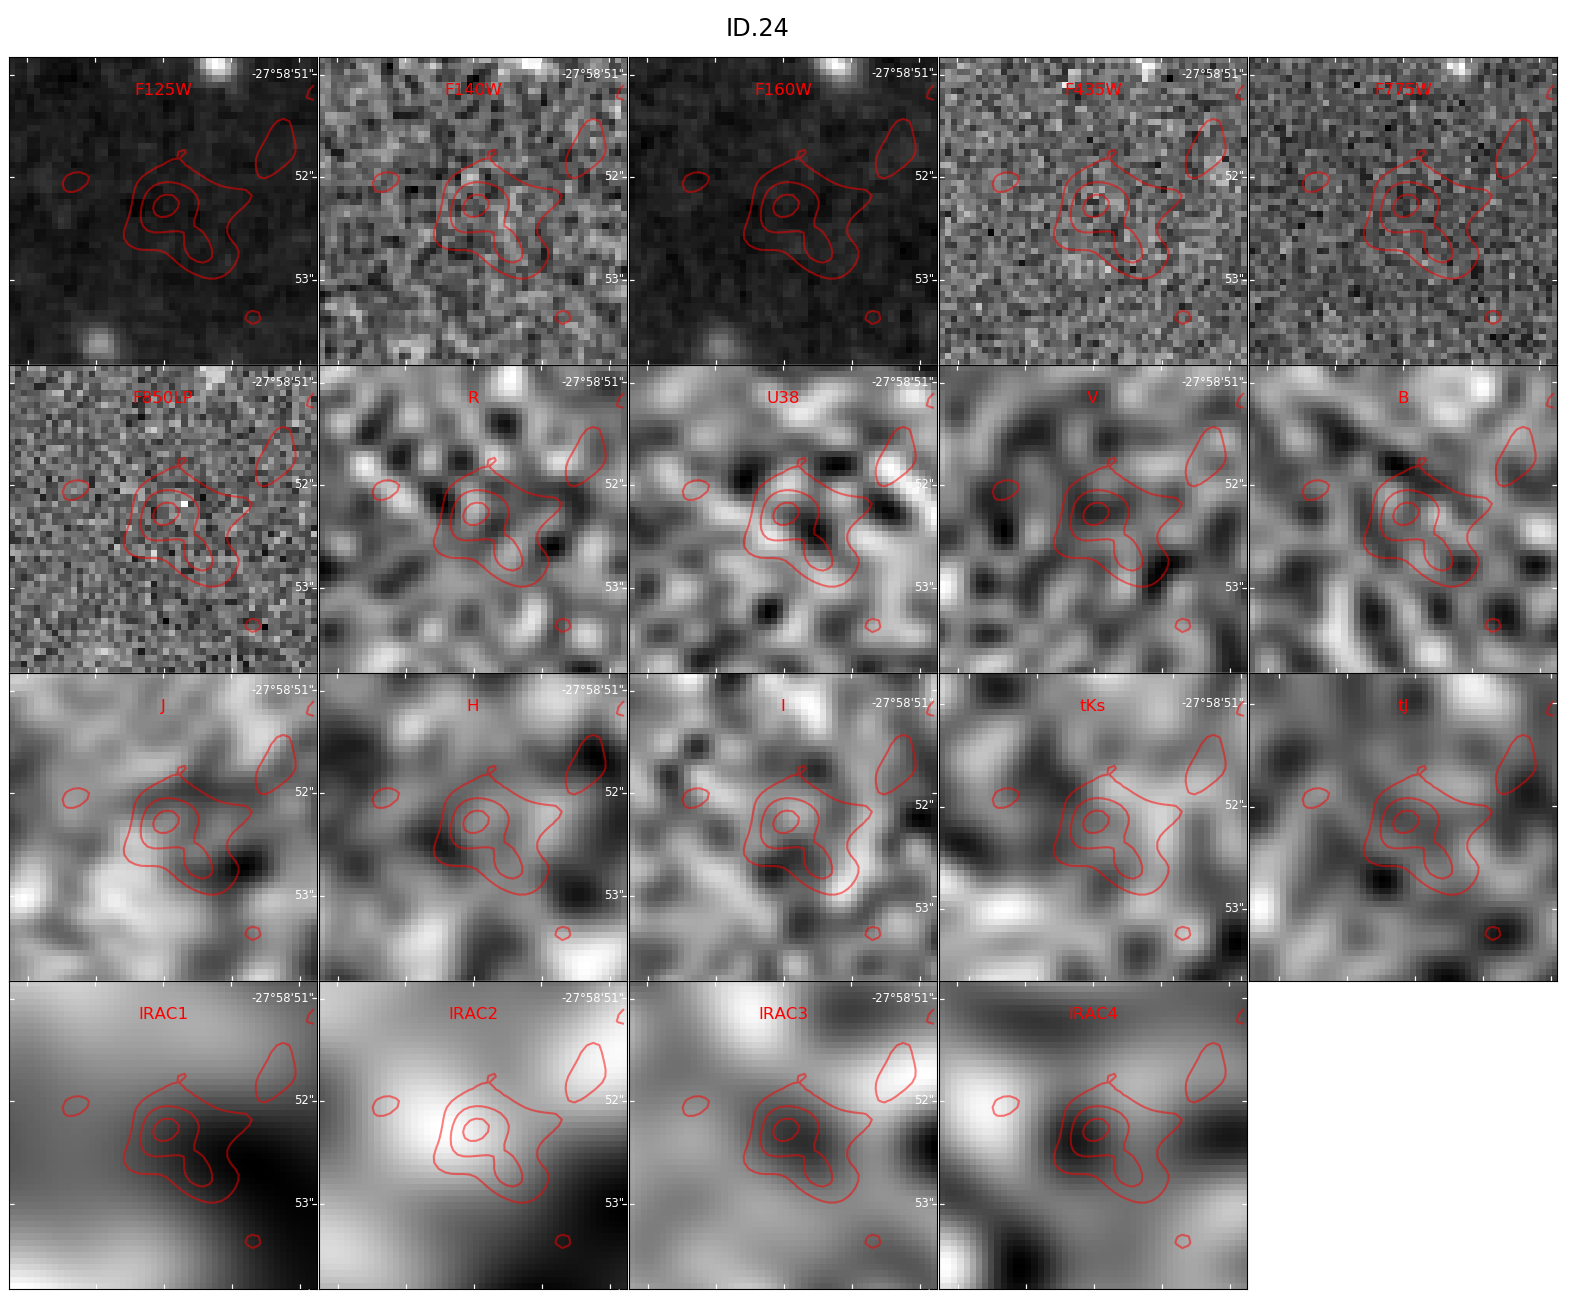
\includegraphics[width=160mm]{Matched/ASPECS_Cutout_23.jpg}
\caption{ID.24. Same contours and cutout size as for \ref{fig:Match_One}.}
\label{fig:Match_Three}
\end{figure}

\begin{figure}[tbp]
\centering 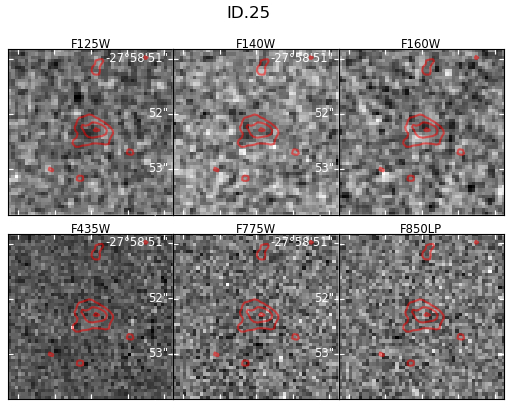
\includegraphics[width=160mm]{Matched/ASPECS_Cutout_24.jpg}
\caption{ID.25. Same contours and cutout size as for \ref{fig:Match_One}.}
\label{fig:Match_Three}
\end{figure}

\begin{figure}[tbp]
\centering 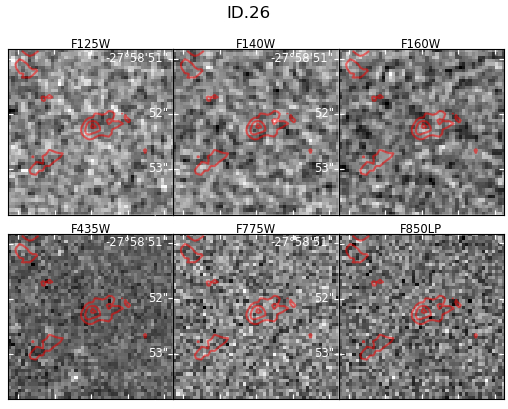
\includegraphics[width=160mm]{Matched/ASPECS_Cutout_25.jpg}
\caption{ID.26. Same contours and cutout size as for \ref{fig:Match_One}.}
\label{fig:Match_Three}
\end{figure}

\begin{figure}[tbp]
\centering 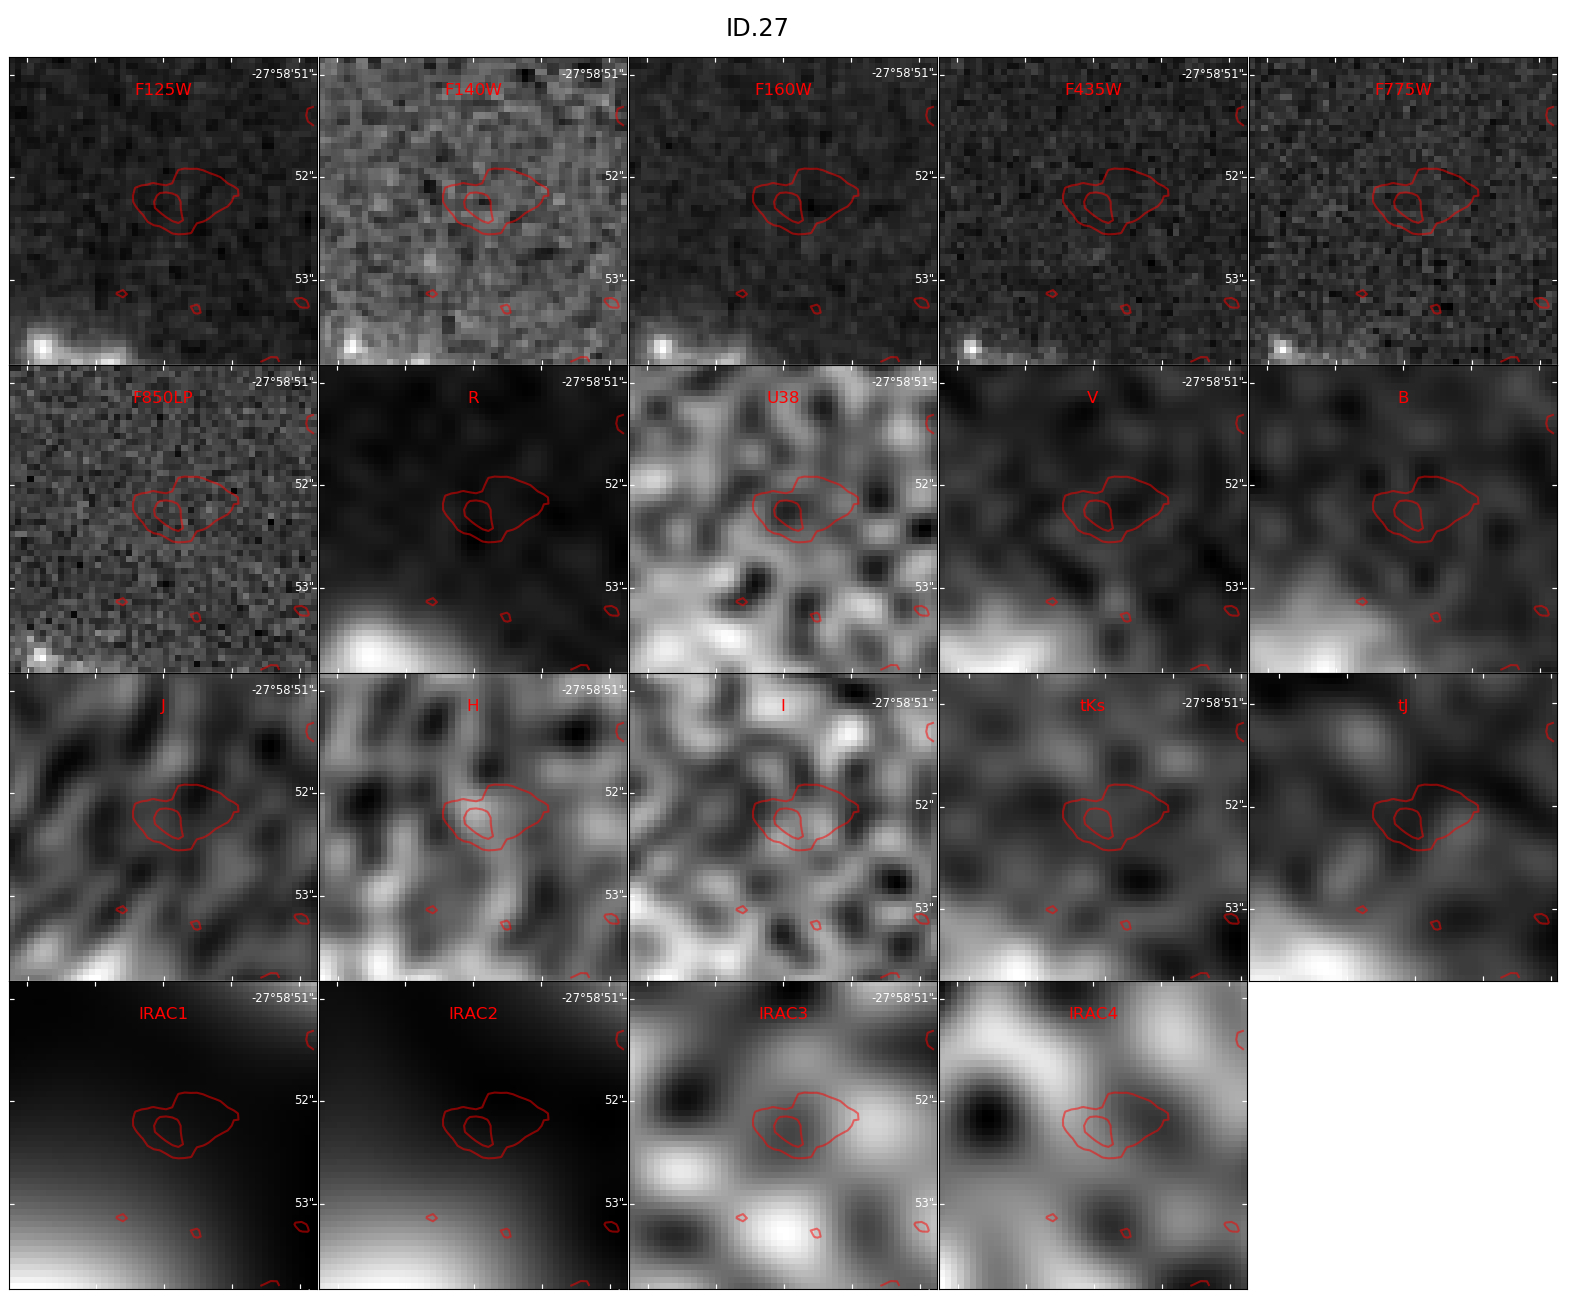
\includegraphics[width=160mm]{Matched/ASPECS_Cutout_26.jpg}
\caption{ID.27. Same contours and cutout size as for \ref{fig:Match_One}.}
\label{fig:Match_Three}
\end{figure}

\begin{figure}[tbp]
\centering 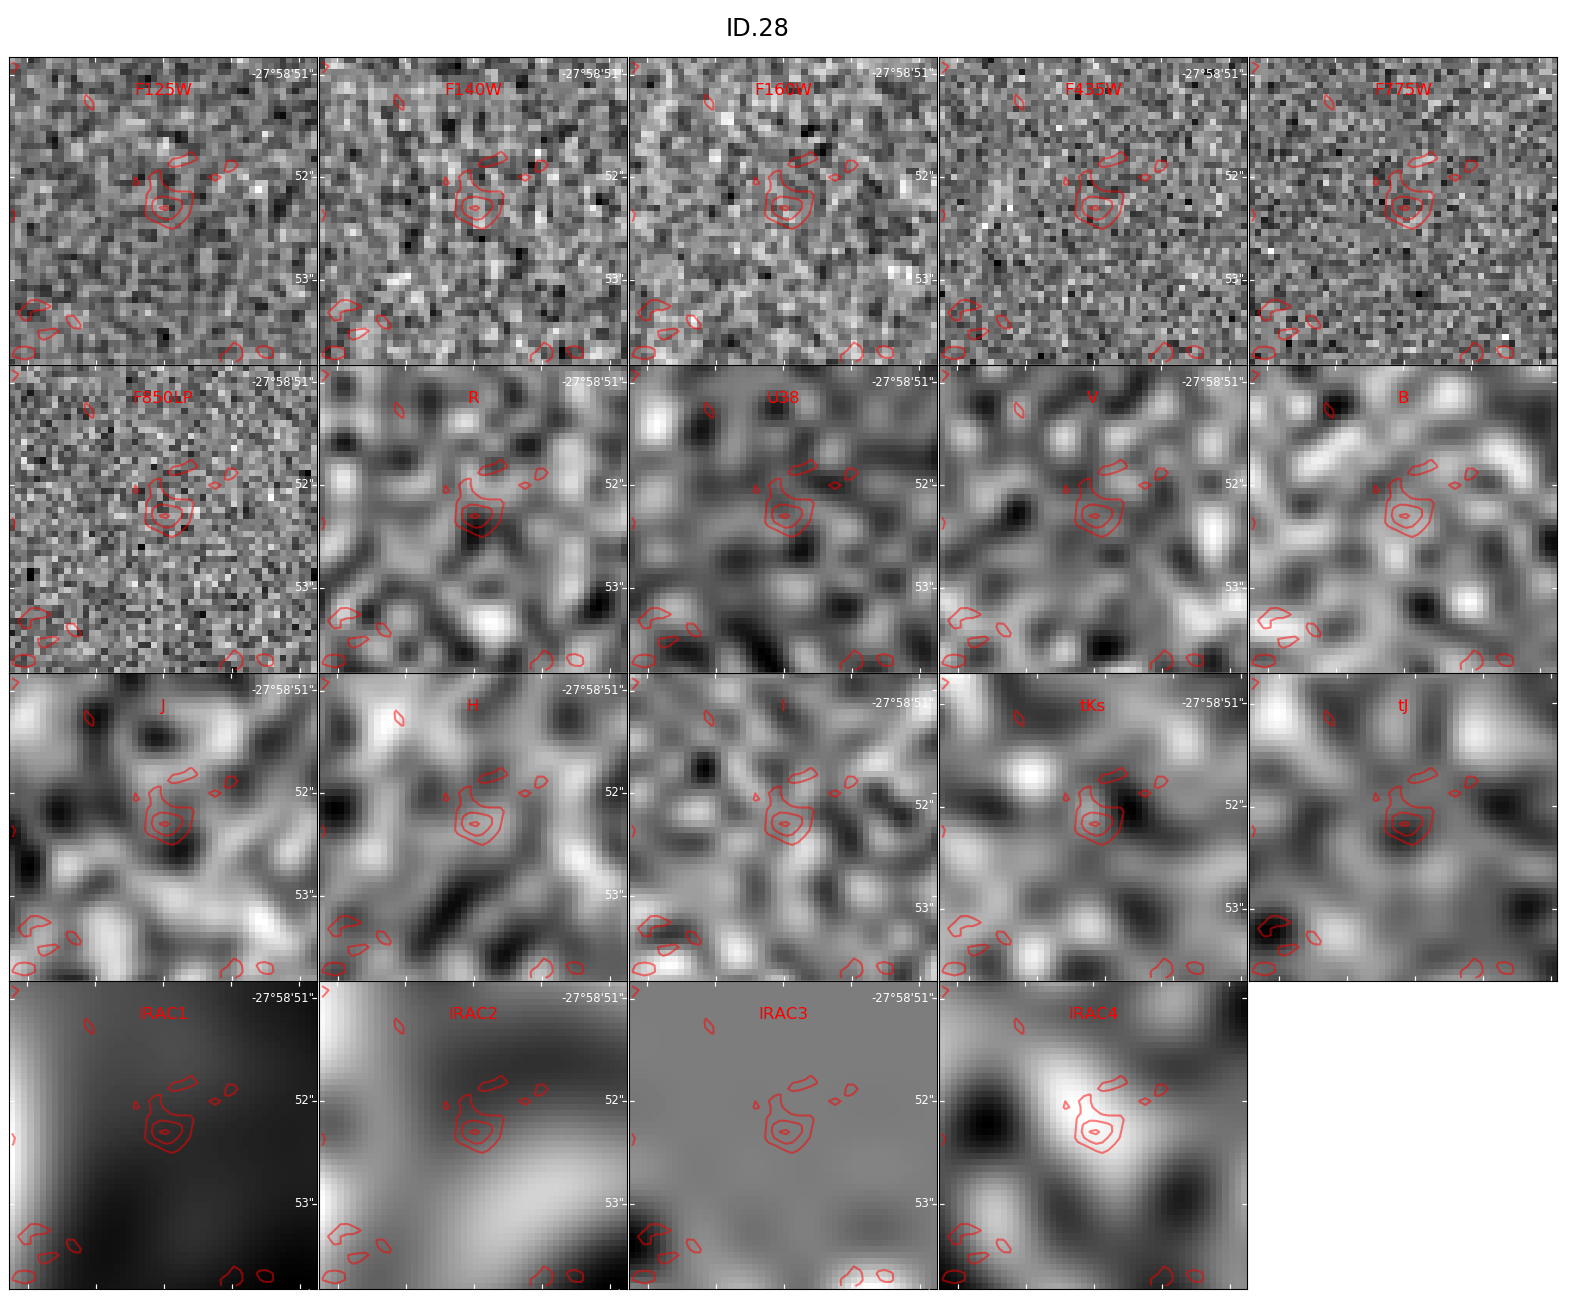
\includegraphics[width=160mm]{Matched/ASPECS_Cutout_27.jpg}
\caption{ID.28. Same contours and cutout size as for \ref{fig:Match_One}.}
\label{fig:Match_Three}
\end{figure}

\begin{figure}[tbp]
\centering 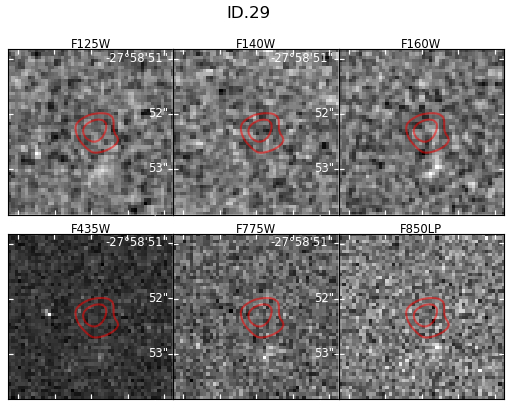
\includegraphics[width=160mm]{Matched/ASPECS_Cutout_28.jpg}
\caption{ID.29. Same contours and cutout size as for \ref{fig:Match_One}.}
\label{fig:Match_Three}
\end{figure}

\begin{figure}[tbp]
\centering 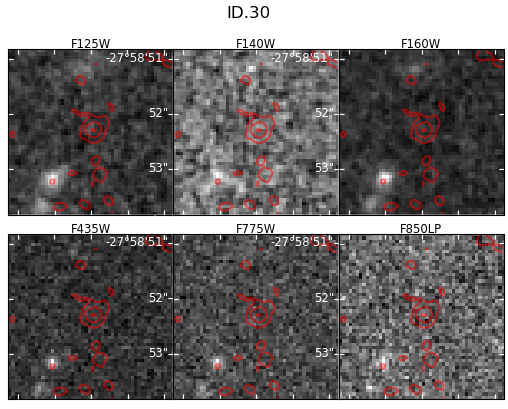
\includegraphics[width=160mm]{Matched/ASPECS_Cutout_29.jpg}
\caption{ID.30. Same contours and cutout size as for \ref{fig:Match_One}.}
\label{fig:Match_Three}
\end{figure}

\begin{figure}[tbp]
\centering 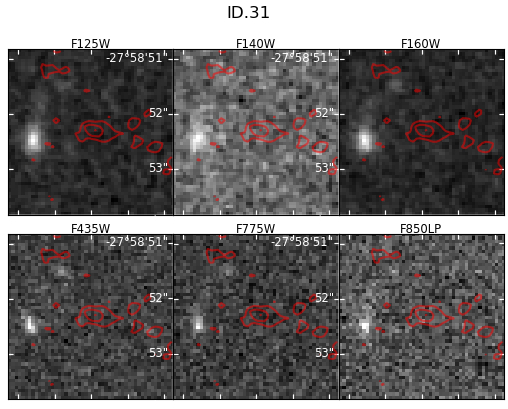
\includegraphics[width=160mm]{Matched/ASPECS_Cutout_30.jpg}
\caption{ID.31. Same contours and cutout size as for \ref{fig:Match_One}.}
\label{fig:Match_Three}
\end{figure}

\begin{figure}[tbp]
\centering 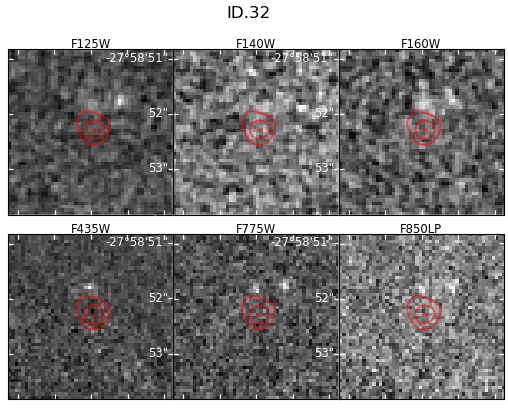
\includegraphics[width=160mm]{Matched/ASPECS_Cutout_31.jpg}
\caption{ID.32. Same contours and cutout size as for \ref{fig:Match_One}.}
\label{fig:Match_Three}
\end{figure}

\begin{figure}[tbp]
\centering 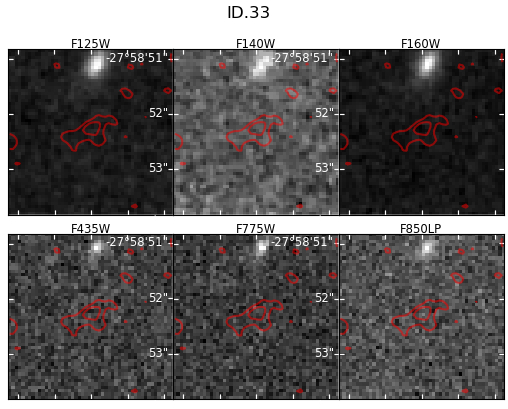
\includegraphics[width=160mm]{Matched/ASPECS_Cutout_32.jpg}
\caption{ID.33. Same contours and cutout size as for \ref{fig:Match_One}.}
\label{fig:Match_Three}
\end{figure}

\begin{figure}[tbp]
\centering 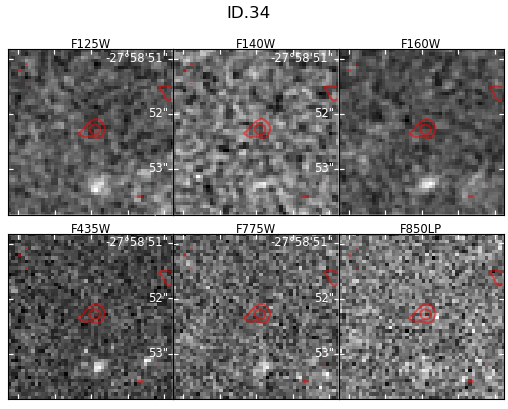
\includegraphics[width=160mm]{Matched/ASPECS_Cutout_33.jpg}
\caption{ID.34. Same contours and cutout size as for \ref{fig:Match_One}.}
\label{fig:Match_Three}
\end{figure}

\begin{figure}[tbp]
\centering 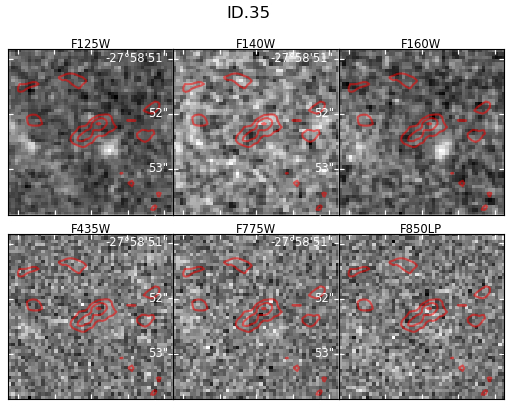
\includegraphics[width=160mm]{Matched/ASPECS_Cutout_34.jpg}
\caption{ID.35. Same contours and cutout size as for \ref{fig:Match_One}.}
\label{fig:Match_Three}
\end{figure}
